\documentclass[aspectratio=169,usenames,dvipsnames]{beamer}

\usepackage{graphicx}
\usepackage{hyperref}
\usepackage{listings}
\usepackage{multimedia}
\usepackage{xcolor}

\title{Using Leaked Data}
\date{}

\begin{document}
\maketitle

\begin{frame}[c]
  \frametitle{Who am I?}

  Not a journalist\pause, but I have talked to a lot of them and I know what
  sort of technical issues they tend to face when dealing with massive troves
  of data.

\end{frame}

\begin{frame}[c]
  \frametitle{Why do I think leaktivism is important?}

  \pause

  The fourth estate relies on confidential sources and leaks to hold
  the powerful accountable.\pause\\Without them the newspapers would just be
  reprinting press releases.

\end{frame}

\begin{frame}[c]
  \frametitle{Why do I think leaktivism is important?}

  \begin{quote}
    That’s the beauty and asymmetry of hacking: with 100 hours of
    work, one person can undo years of work by a multi-million dollar
    company.\\Hacking gives the underdog a chance to fight and win.
  \end{quote}

  \pause

  \centering
  \small
  \href{https://theanarchistlibrary.org/library/hack-back-subcowmandante-marcos-phineas-fisher-hack-back-a-diy-guide-hacking-team}{
    \textcolor{blue}{Hack Back — A DIY Guide (Hacking Team),\\Subcowmandante
    Marcos, Phineas Fisher}}

\end{frame}

\begin{frame}[c]
  \frametitle{Why do I think leaktivism is important?}

  Often it's the only way we can help people nobody else cares about.

\end{frame}

\begin{frame}[c]
  \frametitle{Leaks of past, present and the future}

  Let's use some famous and less known leaks from the distant and
  not-so-distant past as case studies what impact they've had.

\end{frame}

% history section (ancient):
% commission to investigate the FBI
\begin{frame}
  \frametitle{Citizen's Commission to Investigate the FBI}

  \begin{itemize}[<+->]
    \item An early example of "analogue" leaktivism.
    \item Activist group active during the early 1970s.
    \item Broke into an FBI field office during a football game.
    \item Stole over 1,000 classified documents and mailed them to newspapers.
    \item Most news outlets initially reluctant to publish, concerned
      disclosure might compromise ongoing investigations.
  \end{itemize}

\end{frame}

\begin{frame}[c]
  \frametitle{Citizen's Commission to Investigate the FBI}
  Washington Post eventually ran it as a front-page story after verifying
  documents.

  \vspace{1cm}
  \centering

  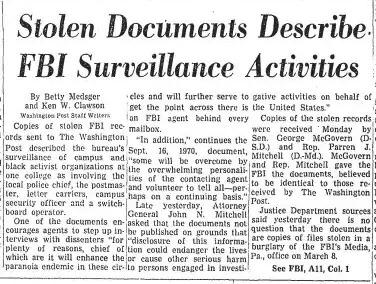
\includegraphics[width=\textwidth,height=0.4\textheight,keepaspectratio]{img/citizens_commission.jpg}
\end{frame}

\begin{frame}[c]
  \frametitle{Citizen's Commission to Investigate the FBI}

  \begin{itemize}[<+->]
    \item Revealed the COINTELPRO operation, a series of covert and illegal
      projects actively aimed at surveilling, infiltrating, discrediting and
      distrupting domestic political organizations.
    \item Exposed documents detailing the FBI's use of postal workers and
      switchboard operators in order to spy on black college students and
      various non-violent black activist groups.
  \end{itemize}
\end{frame}

% early hacking scene
\begin{frame}
  \frametitle{Early hacking scene in 1980s and 1990s}

  \begin{itemize}[<+->]
    \item Early internet was very insecure.
    \item Most early hacking relied on wardialing (calling every phone number
      in an area code sequentially looking for modems.)
    \item And password guessing
    \item Serious, enterprise software used by big corporations and
      governments in those days came with default maintenance and system
      username and passwords.
    \item Hackers scoured manuals in search of those.
    \item Whoever had the best password list was the best hacker.
  \end{itemize}
\end{frame}

\begin{frame}
  \frametitle{Early hacking scene in 1980s and 1990s}

  \centering
  \movie[width=\textwidth,height=0.75\textheight]{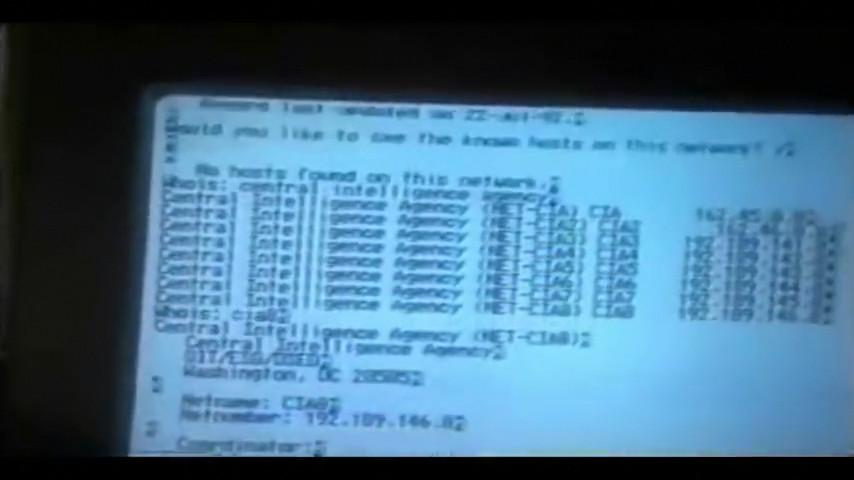
\includegraphics[width=\textwidth,height=0.75\textheight]{img/quantum_leap.jpg}}{img/quantum_leap.mp4}

  \footnotesize
  \href{https://www.youtube.com/watch?v=0a_4IR4v5no&t=74}{\textcolor{blue}{Walk
  on the Wild Side - "Hackers and Phreakers" (1994, Channel 4 UK)}}
\end{frame}

\begin{frame}
  \frametitle{Early hacking scene in 1980s and 1990s}

  \begin{itemize}[<+->]
    \item Most people did it just for fun and thrills.
    \item In those days the only way to learn about hacking, telecom and
      enterprise systems was to break into them.
    \item There weren't any educational materials for people to learn
      "ethical" hacking in a legal way.
    \item Lots of corporate, government, military, intelligence access.
    \item It hasn't crossed anybody's mind yet that the data they had access
      to could have political or journalistic impact.
  \end{itemize}
\end{frame}

\begin{frame}
  \frametitle{Early hacking scene in 1980s and 1990s}

  \centering

  \movie[width=\textwidth,height=0.75\textheight]{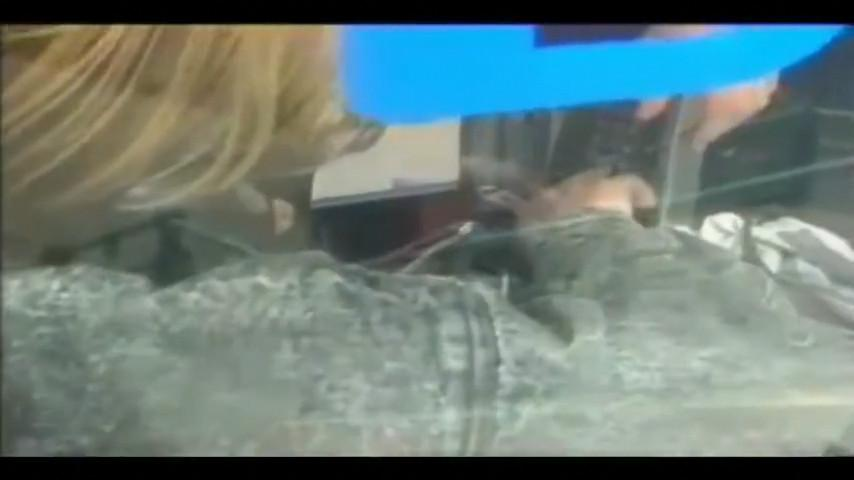
\includegraphics[width=\textwidth,height=0.7\textheight]{img/traced.jpg}}{img/traced.mp4}

  \footnotesize
  \href{https://www.youtube.com/watch?v=0a_4IR4v5no&t=770}{\textcolor{blue}{Walk
  on the Wild Side - "Hackers and Phreakers" (1994, Channel 4 UK)}}
\end{frame}

% china/indonesia
\begin{frame}
  \frametitle{Early hacking scene in 1980s and 1990s}

  \begin{itemize}[<+->]
    \item The term "hacktivism" coined by the Cult of the Dead Cow in their
      \href{https://blog.9while9.com/manifesto-anthology/2001.html}{\textcolor{blue}{Hacktivismo
      Declaration}} in 2001.
    \item Although I did find the word in
      \href{https://en.wikipedia.org/wiki/The_Cuckoo's_Egg_(book)}{\textcolor{blue}{a book from
      1989}}.
    \item The cDc is a group we would today describe as early "grey-hat
      hackers," exploiting systems to report the vulnerabilities and get them
      fixed.
    \item They were against website defacements, distributed denial of service
      and other malicious attacks.
    \item Not the political "hacktivism" of today.
    \item Politically motivated hacking did already exist.
    \item Focused on defacing websites with politically motivated messages.
  \end{itemize}
\end{frame}

\begin{frame}[c]
  \frametitle{Early hacking scene in 1980s and 1990s}

  \centering

  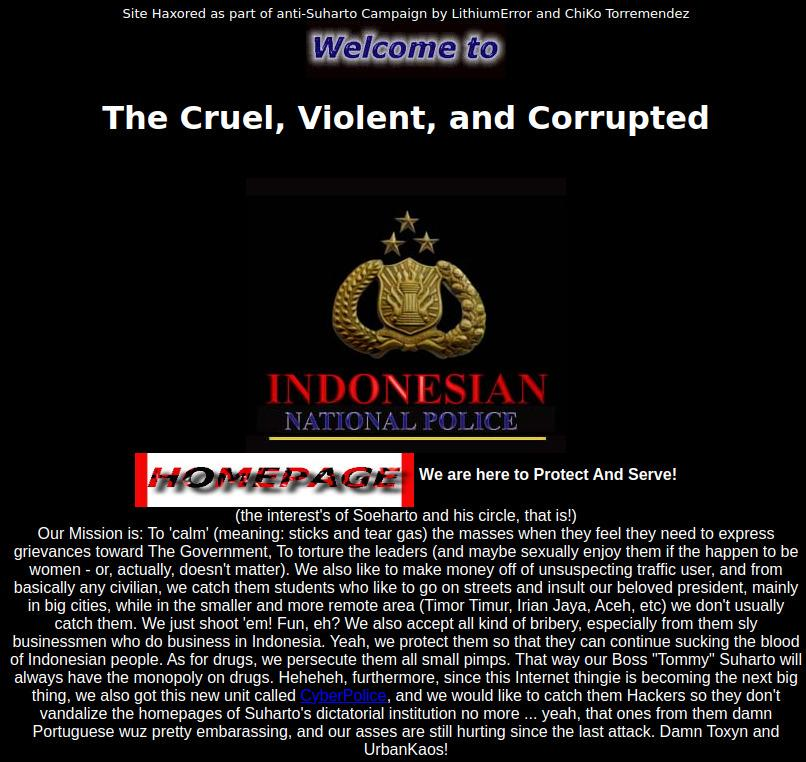
\includegraphics[width=\textwidth,height=0.75\textheight,keepaspectratio]{img/kepolisian_republik.jpg}

  \footnotesize
  \href{https://www.2600.com/hackedphiles/timor011998/indo3/}{\textcolor{blue}{\emph{Indonesian
  Police Force website defaced during student protests of 1998}}}
\end{frame}

\begin{frame}[b]
  \frametitle{Early hacking scene in 1980s and 1990s}

  \centering

  
\includegraphics[width=\textwidth,height=0.6\textheight,keepaspectratio]{img/honkers_union.png}

  \footnotesize
  \emph{Website defaced by early Chinese "hacktivist" group
  "\href{https://en.wikipedia.org/wiki/Honker_Union}{\textcolor{blue}{Honker Union}}"
  with a pro-Chinese government nationalist message}
  \vspace{1cm}
\end{frame}

% leaking mailspools
\begin{frame}
  \frametitle{Early hacking scene in 1980s and 1990s}

  \begin{itemize}[<+->]
    \item There was fierce competition and machoism between hacker groups.
    \item One of the best (worst) ways to embarass a competing hacker crew was
      to leak and publish their personal emails, termed "dumping mailspools."
    \item Probably the closest thing to the "hack-and-leak" operations of
      today.
    \item There is also lineage to warez and piracy groups.
    \item Most hackers did it just for fun, did not see the value in the data
      they were able to access.
    \item The few who did could not get journalists interested.
    \item The bandwidth and storage we take for granted today also did not
      exist back then.
  \end{itemize}

\end{frame}

\begin{frame}
  \frametitle{Early hacking scene in 1980s and 1990s}

  \centering

  \movie[width=\textwidth,height=0.75\textheight]{
\includegraphics[width=\textwidth,height=0.7\textheight]{img/black_hats_world.jpg}}{img/black_hats_world.mp4}

  \footnotesize
  \href{https://www.youtube.com/watch?v=aSSqLLeGdHI&t=323}{\textcolor{blue}{Hackers in Wonderland  (2000, Russel Barnes)}}
\end{frame}

% karl koch
\begin{frame}
  \frametitle{Karl Koch}

  \begin{itemize}[<+->]
    \item One exception was German hacker
      \href{https://en.wikipedia.org/wiki/Karl_Koch_\%28hacker\%29}{\textcolor{blue}{Karl Koch
      aka "hagbard"}}.
    \item Gained access to United States military computers in 1986.
    \item Tried selling information to journalists, but they were not
      interested.
    \item Travelled to Eastern Germany to sell the information to the Soviets.
    \item Caused the "Cold War Computer Espionage Incident."
    \item Eventually got caught and died in mysterious circumstances.
  \end{itemize}

\end{frame}

\begin{frame}[c]
  \frametitle{Karl Koch}

  \centering

  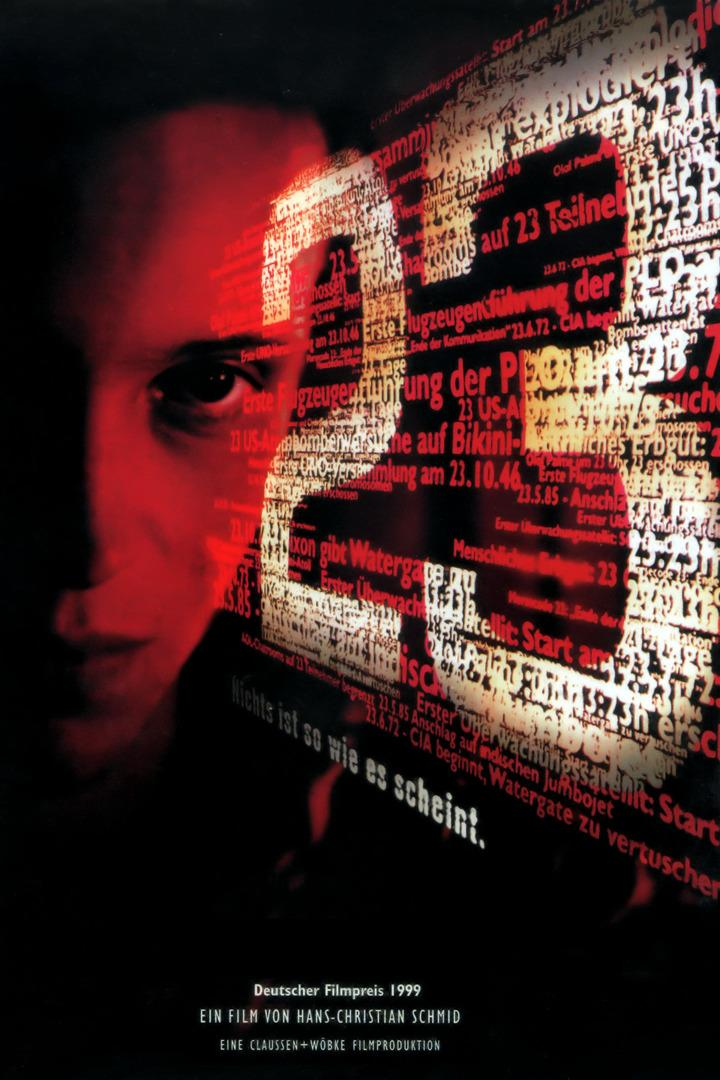
\includegraphics[width=\textwidth,height=0.75\textheight,keepaspectratio]{img/23.jpg}

  \footnotesize
  \href{https://www.imdb.com/title/tt0126765/}{\textcolor{blue}{23 (1998)}}
\end{frame}

% jeremy hammond
\begin{frame}
  \frametitle{Early 2000s}

  \begin{itemize}[<+->]
    \item The security industry goes "legit."
    \item Full disclosure, shift in software industry culture, and bug
      bounties provide economic incentive for hackers to turn "white hat" and
      report the vulnerabilities they find.
    \item FBI propaganda and high-profile arrests like Kevin Mitnick also
      played a role in the black hat scene dying down.
    \item The remaining black hats turned to monetary motives like
      carding, fraud and selling data.
  \end{itemize}
\end{frame}

\begin{frame}[c]
  \frametitle{Early 2000s}

  \centering

  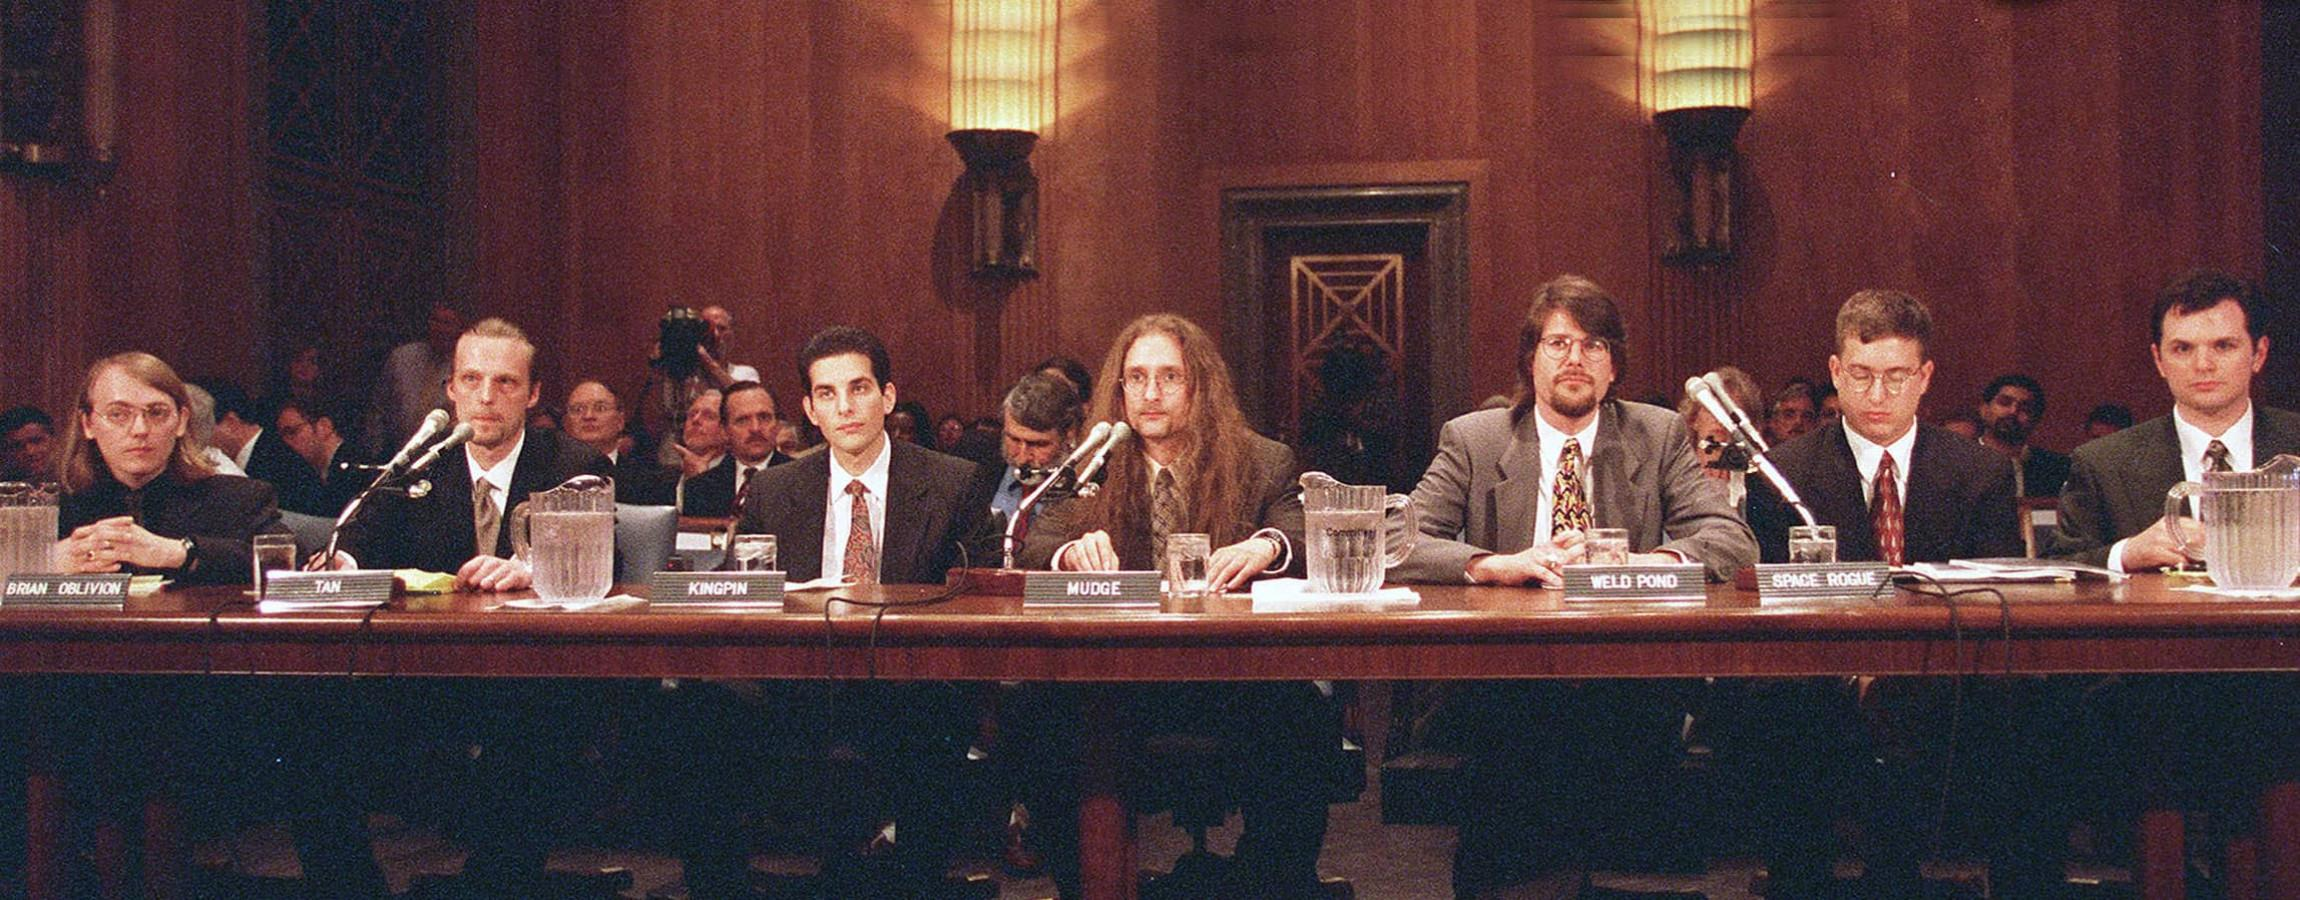
\includegraphics[width=\textwidth,height=0.75\textheight,keepaspectratio]{img/l0pht_congress.jpg}

  \footnotesize
  \emph{mudge and other members of the cDc and the l0pht testifying in front
  of congress, wearing suits}
\end{frame}

%% hackthissite
\begin{frame}
  \frametitle{HackThisSite}
  \framesubtitle{\url{https://www.hackthissite.org/}}

  \begin{itemize}[<+->]
    \item There were now many sites where aspiring hackers could sign up and
      solve a series of challenges to hone their skills legally.
    \item One of the more popular of such sites was HackThisSite.
    \item Unlike the others, the challenges on HackThisSite had a distinct
      anarchist, leftist political flavour.
    \item For example, one of the challenges on the site tasked you with
      hacking into a faux replica of a neo-nazi fascist group's website and
      getting access to their member list.
  \end{itemize}

\end{frame}

%% jeremy hammond
\begin{frame}
  \frametitle{Jeremy Hammond}

  HackThisSite was founded by American anarchist and former computer hacker
  \href{https://en.wikipedia.org/wiki/Jeremy_Hammond}{\textcolor{blue}{Jeremy
  Hammond}}.

  \centering

  
\includegraphics[width=\textwidth,height=0.7\textheight,keepaspectratio]{img/jeremy_hammond.jpg}

\end{frame}

\begin{frame}[c]
  \frametitle{Jeremy Hammond}

  \centering

  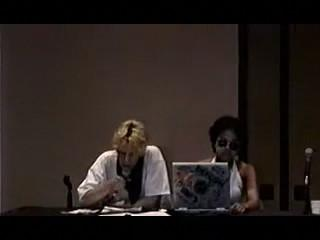
\includegraphics[width=\textwidth,height=0.75\textheight,keepaspectratio]{img/jeremy_hammond_defcon.jpg}

  \footnotesize
  \href{https://www.youtube.com/watch?v=UeZjWdg_Qn8}{\textcolor{blue}{Jeremy Hammond - DEFCON 12 (2004)}}
\end{frame}

%% scientology leaks
\begin{frame}[c]
  \frametitle{Anonymous}

  In 2008, protests against the Church of Scientology were organized by a
  group calling themselves Anonymous.

\end{frame}

\begin{frame}[c]
  \frametitle{Anonymous}

  \centering

  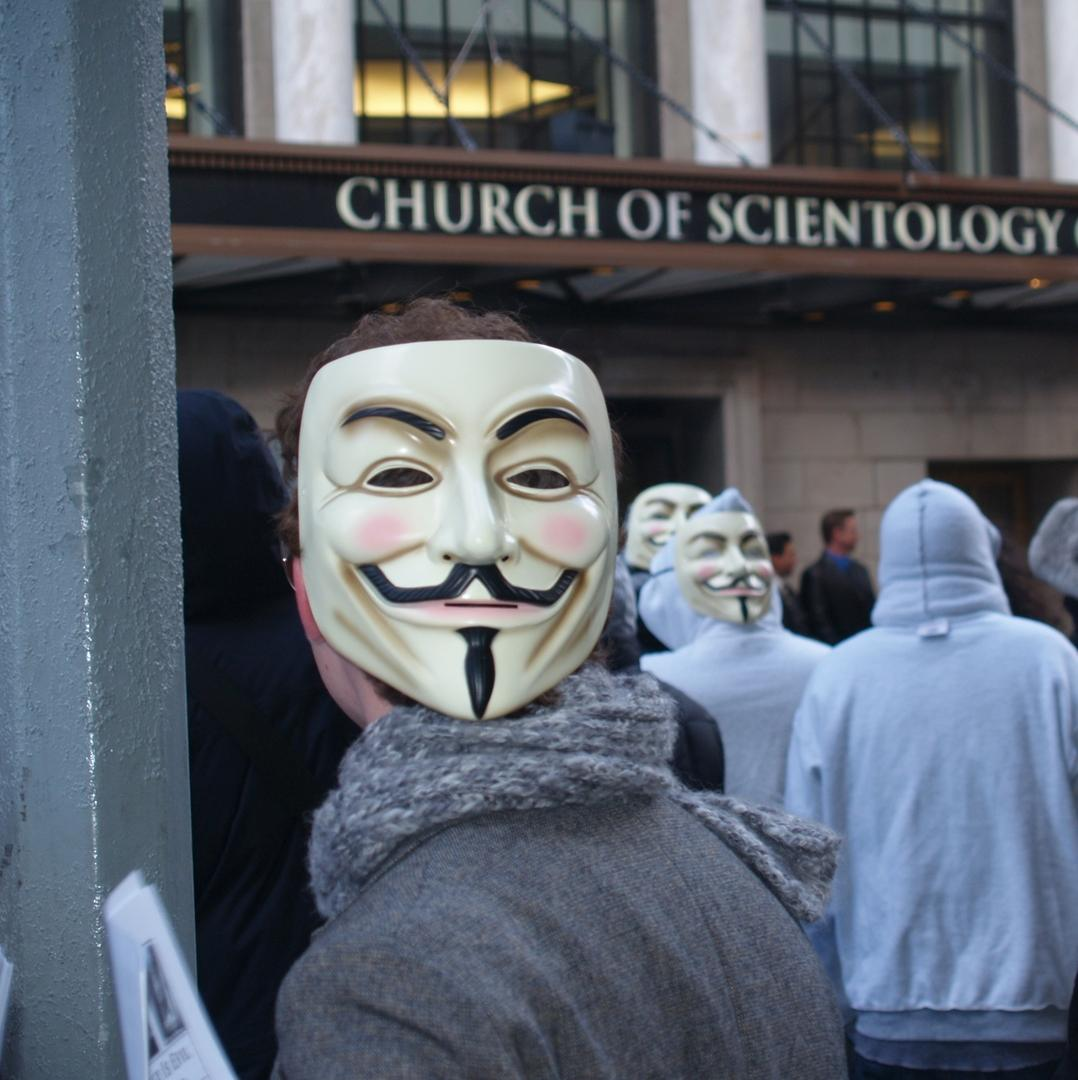
\includegraphics[width=\textwidth,height=0.7\textheight,keepaspectratio]{img/anonymous.jpg}

  \footnotesize
  \emph{A member of the group Anonymous during a real life protest against the
  Church of Scientology (Image Attribution: David Shankbone)}

\end{frame}

\begin{frame}
  \frametitle{Anonymous}

  \begin{itemize}[<+->]
    \item Protests against the Church of Scientology happened both online and
      offline.
    \item The Church restricted information based on its member ranking
      within the organization (based on how much money they've
      donated.)
    \item One of the actions taken by Anonymous was to release all church
      documents and stories accessible only to high ranking members.
    \item Earliest example of organized hack-and-leak campaign by Anonymous.
    \item Followed by release of Sarah Palin's personal emails.
    \item Anonymous involvement in real-life protests later continued with the
      Occupy Wall Street movement.
  \end{itemize}

\end{frame}

%% latvia bank leak (2010)
\begin{frame}
  \frametitle{Latvia Banking Leaks (2010)}
  \framesubtitle{\url{https://www.theregister.com/2010/05/14/latvian_hacker_whistleblower/}}

  \begin{itemize}[<+->]
    \item In 2010, a hacker calling himself Neo started releasing embarassing
      infomation such as bonuses received by bank managers during a bail-out
      caused by the financial crisis.
    \item The hacker was identified as a lone artificial intelligence
      researcher working at an university.
    \item He was pardoned for his actions by the country's president.
    \item Unprecedented hacktivism for its political impact.
  \end{itemize}

\end{frame}
%% most hacker anthropology is anglocentric
\begin{frame}[c]

  \centering

  hacker anthropology is a very anglocentric field

\end{frame}

%% history section (wikileaks era)
%% wikileaks
\begin{frame}[c]
  \frametitle{Wikileaks Era}

  \centering

  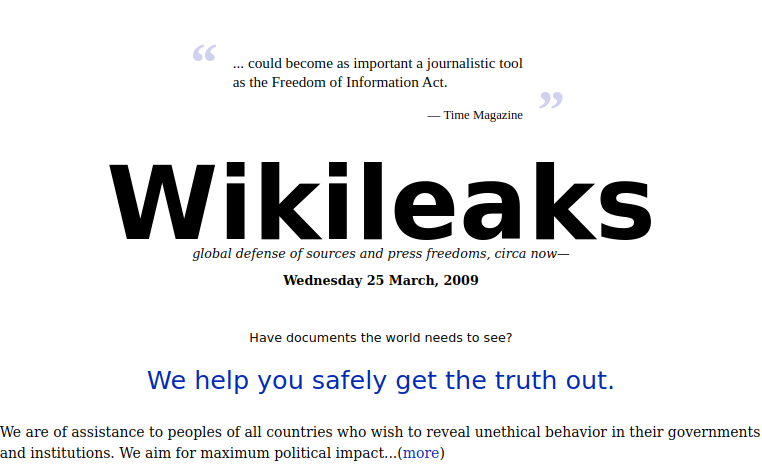
\includegraphics[width=\textwidth,height=0.5\textheight,keepaspectratio]{img/wikileaks.png}

  \vspace{5mm}

  \footnotesize
  \emph{A screenshot of the early wikileaks.org homepage}
\end{frame}

\begin{frame}
  \frametitle{Wikileaks Era}

  \begin{itemize}[<+->]
    \item Founded by Australian Julian Assange, a former Australian hacker
      under the handle mendax.
    \item Arrested for hacking into the United States Department of Defense in
      his youth and attempting to leak the information to the press, sentenced
      to a fine.
    \item Based on the idea that strong cryptography and a document dropbox
      running on top of the Tor network can enable mass anonymous leaking of
      confidential documents and protect sources.
    \item This infrastructure was engineered by a mysterious, anonymous figure
      calling themselves "the Architect."
  \end{itemize}

\end{frame}
%% chelsea manning (2010)
\begin{frame}[c]
  \frametitle{Collateral Murder (2010)}

  \centering

  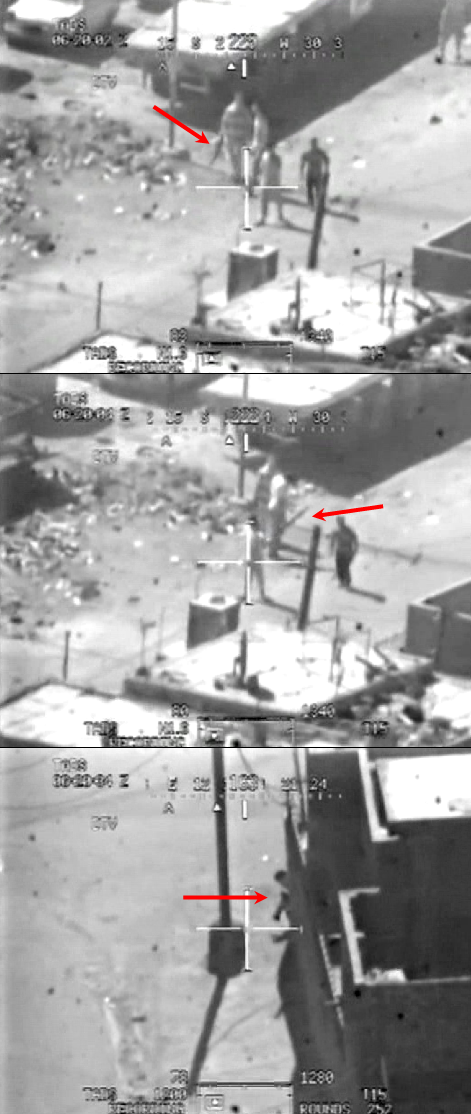
\includegraphics[width=\textwidth,height=0.7\textheight,keepaspectratio]{img/collateral_murder.png}

  \footnotesize
  \emph{Stills from a video released by WikiLeaks, showing an US attack
  helicopter shooting innocent civilians in Iraq}
\end{frame}

%% cables leak (2010)
\begin{frame}
  \frametitle{United States diplomatic cables leak (2010)}
  \framesubtitle{\url{https://ddosecrets.com/wiki/Cablegate}}

  \begin{itemize}[<+->]
    \item In November 2010, WikiLeaks released a cache of classified cables
      sent by the U.S State Departments between its consulates, embassies and
      diplomatic missions around the world.
    \item Redacted cables were published by a consortium of journalists from
      various publications around the world.
    \item Unredacted version of the data was released by WikiLeaks as an
      encrypted "insurance file," the password to which was later published in
      a book by one of the journalists who worked on the cables' release.
  \end{itemize}

\end{frame}

\begin{frame}[c]
  \frametitle{Chelsea Manning}
  \framesubtitle{\url{https://twitter.com/xychelsea}}

  \centering

  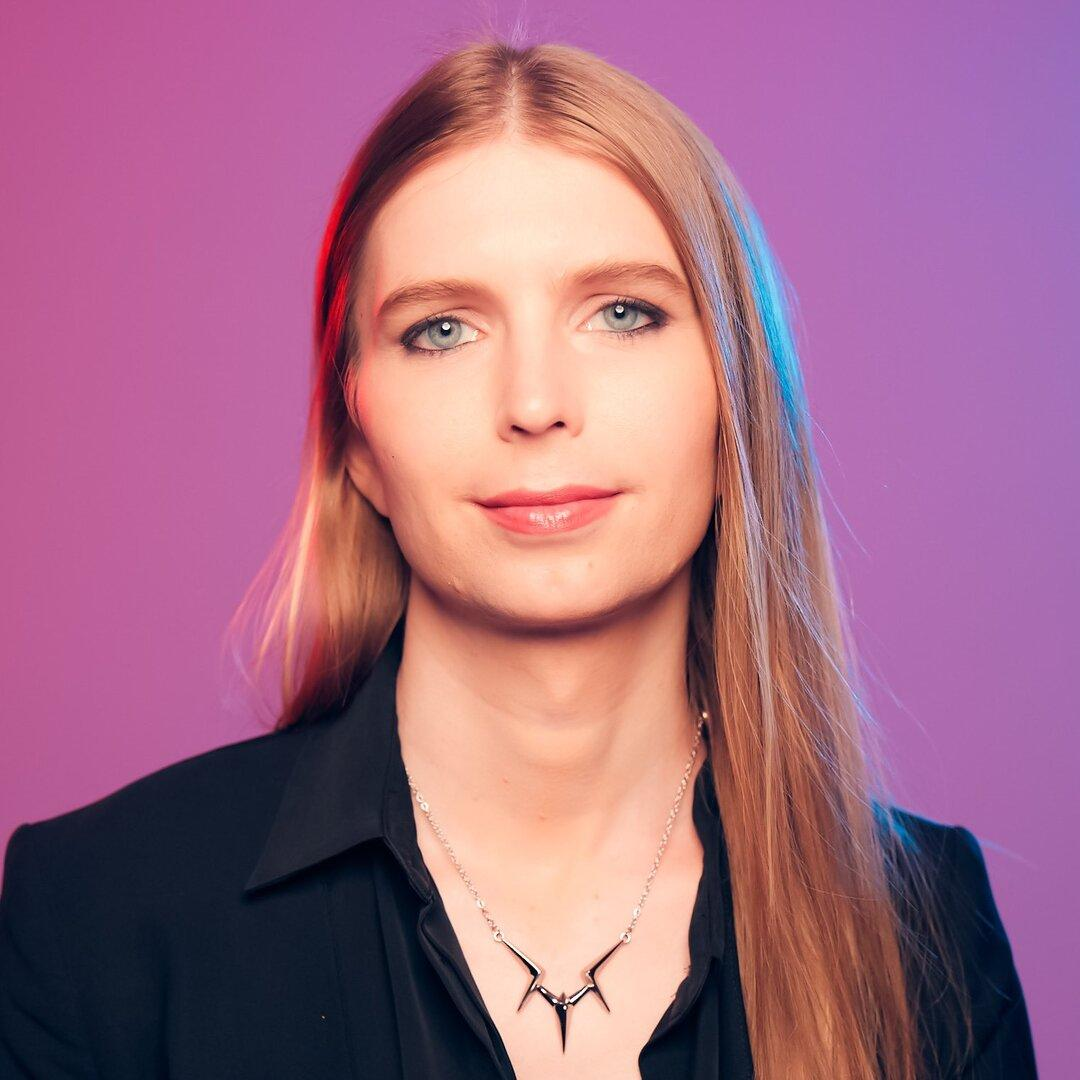
\includegraphics[width=\textwidth,height=0.75\textheight,keepaspectratio]{img/chelsea_manning.jpg}

  \footnotesize
  \emph{Photo of Chelsea Manning in 2022, Creative Commons, Credit: Matt
  Barnes}
\end{frame}

\begin{frame}
  \frametitle{Chelsea Manning}
  \framesubtitle{\url{https://twitter.com/xychelsea}}

  \begin{itemize}[<+->]
    \item The alleged source of documents was Chelsea Manning, at the time
      serving in the U.S. army in Iraq.
    \item Confided to a friend, Adrian Lamo, that she was the source of the
      leaks, who reported her to the authorities.
    \item Sentenced to thirty-five years imprisonment under the Espionage Act.
    \item Released in 2017 after her sentence was commuted by Barack Obama.
  \end{itemize}

\end{frame}

%% stratfor (2011)
\begin{frame}[c]
  \frametitle{LulzSec (2011)}

  In 2011, a few more skilled members who participated in the previous
  Anonymous actions organized into a smaller black hat hacking crew called
  Lulz Security and started wrecking havoc across the internet.

  \centering

  \vspace{1cm}

  
\includegraphics[width=\textwidth,height=0.3\textheight,keepaspectratio]{img/lulzsec.png}

\end{frame}

\begin{frame}
  \frametitle{Operation AntiSec (2011)}

  \begin{itemize}[<+->]
    \item Together with Anonymous and other hacking groups, LulzSec launched
      Operation AntiSec or Anti-Security.
    \item They voiced their opposition to the professional white-hat
      information security industry, calling them out as frauds, sell-outs
      and charlatans.
    \item And spearheaded a series of politically-motivated, anarchist
      hacking actions against law enforcement and the intelligence community
      during the height of the Occupy Wall Street movement.
    \item For more background on the group's motivations, I recommend
      reading the \emph{"Lines in the Sand: Which Side Are You On in the
      Hacker Class War"} article in issue 68 of the Phrack zine.
    \item \url{http://phrack.org/issues/68/16.html}
  \end{itemize}

\end{frame}

\begin{frame}
  \frametitle{Stratfor (2011)}
  \framesubtitle{\url{https://ddosecrets.com/wiki/Stratfor_emails}}

  \begin{itemize}[<+->]
    \item In December 2011, Anti-Sec claimed responsibility for a hack on
      private intelligence company Stratfor (Strategic Forecasting.)
    \item Data on the company's clients, including credit card information and
      emails was provided to WikiLeaks.
    \item At this point one of the group's members, Hector Xavier Monsegur
      (sabu) was compromised and working as an FBI informant.
    \item The members of the group were arrested shortly thereafter.
    \item Jeremy Hammond was sentenced to ten years in federal prison for his
      role in the action.
  \end{itemize}

\end{frame}

\begin{frame}
  \frametitle{Stratfor (2011)}
  \framesubtitle{\url{https://ddosecrets.com/wiki/Stratfor_emails}}

  The same Jeremy Hammond who founded HackThisSite.

  \vspace{5mm}

  \centering

  
\includegraphics[width=\textwidth,height=0.6\textheight,keepaspectratio]{img/jeremy_hammond.jpg}

\end{frame}

\begin{frame}[c]

  \centering

  People got arrested.
  \pause\hspace{1mm}People got scared.
  \pause\hspace{1mm}Anonymous was over.
  \pause\hspace{1mm}Hacktivism was over.
  \pause\hspace{1mm}Leaking was over.

\end{frame}

\begin{frame}[c]

  \centering

  
\includegraphics[width=0.6\textwidth,height=0.6\textheight,keepaspectratio]{img/cant_arrest_an_idea.png}

  \vfill

  \footnotesize
  \emph{tweet from Topiary, one of the arrested LulzSec members, "you cannot
  arrest an idea"}
\end{frame}

\begin{frame}[c]
  \frametitle{Julian Assange claims asylum (2012)}

  \centering
  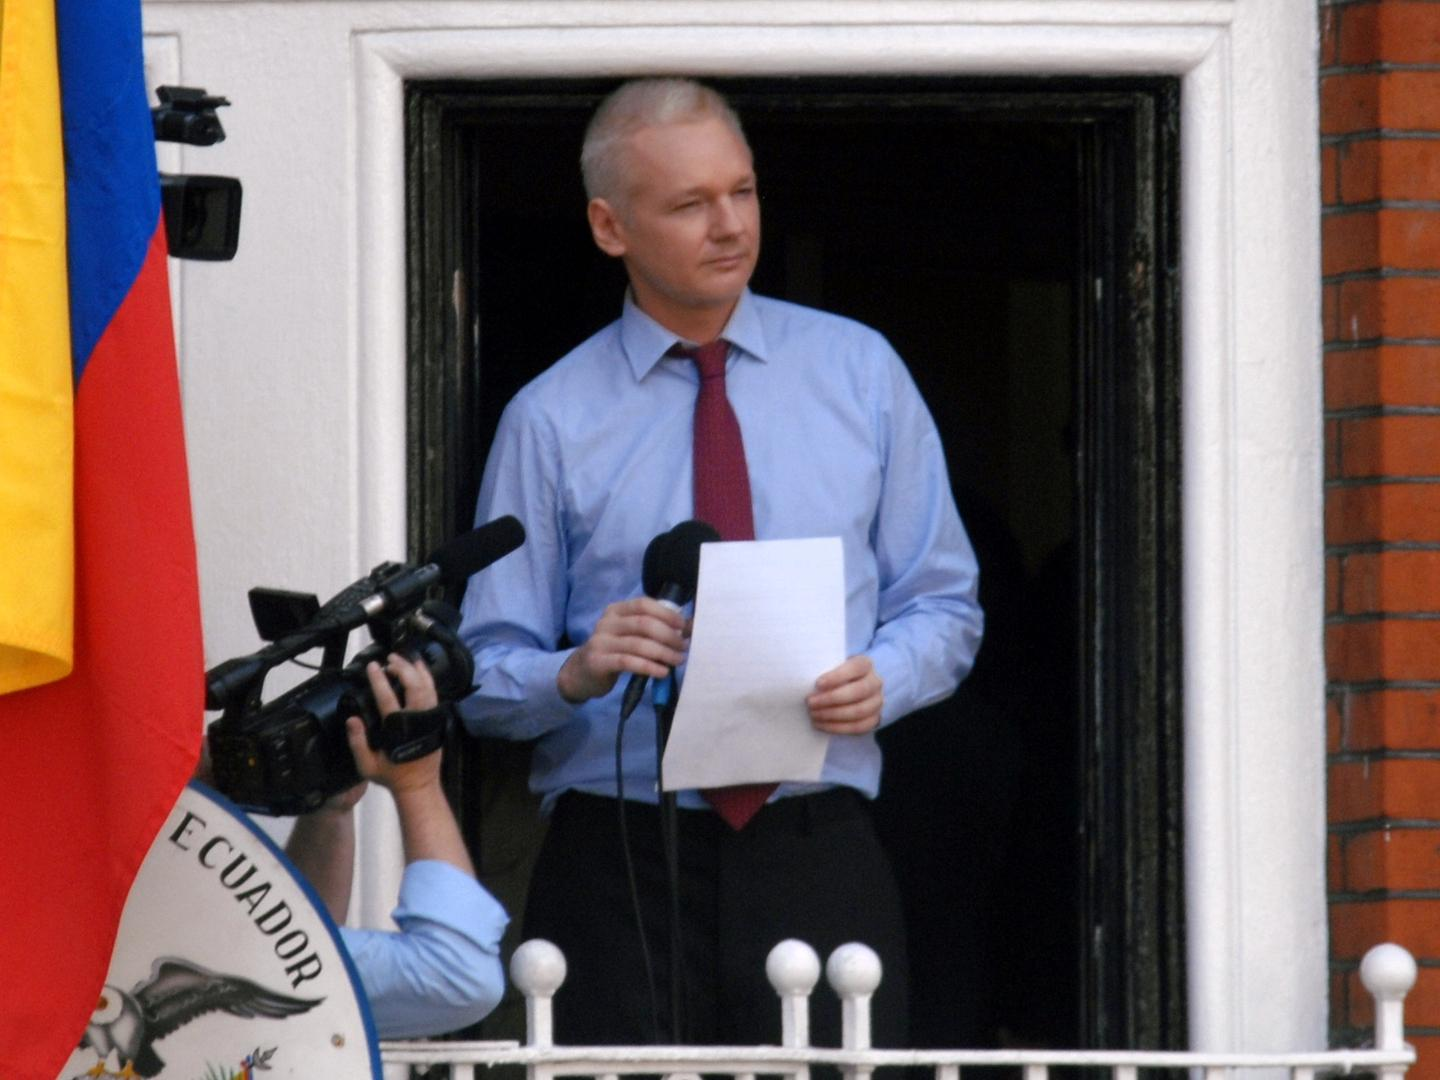
\includegraphics[width=\textwidth,height=0.5\textheight,keepaspectratio]{img/julian_embassy.jpg}

  \vspace{5mm}

  \footnotesize
  \emph{Assange on the balcony of Ecuadorian embassy in London in 2012}
\end{frame}

%% syria files (2012)
\begin{frame}
  \frametitle{Syria Files (2012)}
  \framesubtitle{\url{https://ddosecrets.com/wiki/Syria_files}}

  In July 2012, WikiLeaks began publishing Syria Files, a collection of
  more than two million emails from Syrian political figures and ministries
  dating from August 2006 to March 2012.

  \pause

  \begin{itemize}[<+->]
    \item Hacktivist group RevoluSec have taken credit for the leak in
      conjunction with Anonymous claiming to have access to all Syrian
      internet routers and switches.
    \item Uncovered western companies continuing to supply
      the Syrian regime with telecommunications equipment.
    \item Public relations firm Brown Lloyd James sending an email to Syrian
      authorities offering advice on how to repress the uprising.
    \item Led to more sanctions against the Bashar al-Assad regime.
    \item Other interesting actions took place around this time, for example,
      Telecomix supplying Syrian people with dialup internet access during
      government internet shutdowns.
  \end{itemize}
\end{frame}

%% offshore leaks (2013)
\begin{frame}
  \frametitle{Offshore Leaks (2013)}
  \framesubtitle{\url{https://offshoreleaks.icij.org/}}

  Offshore leaks was a report disclosing details of 130,000 offshore acounts
  that came out in April 2013.

  \pause
  \vspace{5mm}

  \begin{itemize}[<+->]
    \item Led to the formation of the International Consortium of
      Investigative Journalists (ICIJ).
    \item With ICIJ, came a more closed model of leaking, publishing
      editorialised reports without releasing the complete source material.
    \item Contradictory to the "scientific journalism" model enabled by
      WikiLeaks model of full disclosure of source data.
  \end{itemize}

\end{frame}

%% securedrop
\begin{frame}
  \frametitle{SecureDrop (2013)}
  \framesubtitle{\url{https://securedrop.org/}}

  SecureDrop is a free software platform for secure communication between
  journalists and sources initially developed by Aaron Swartz.\\2013 saw the
  launch of the first SecureDrop instance by the New Yorker.\\Since then, it
  has allowed other publications to operate their own secure whistleblowing
  dropboxes to receive leaked documents without the involvement of an
  intermediary like WikiLeaks.

  \vspace{2mm}

  \centering

  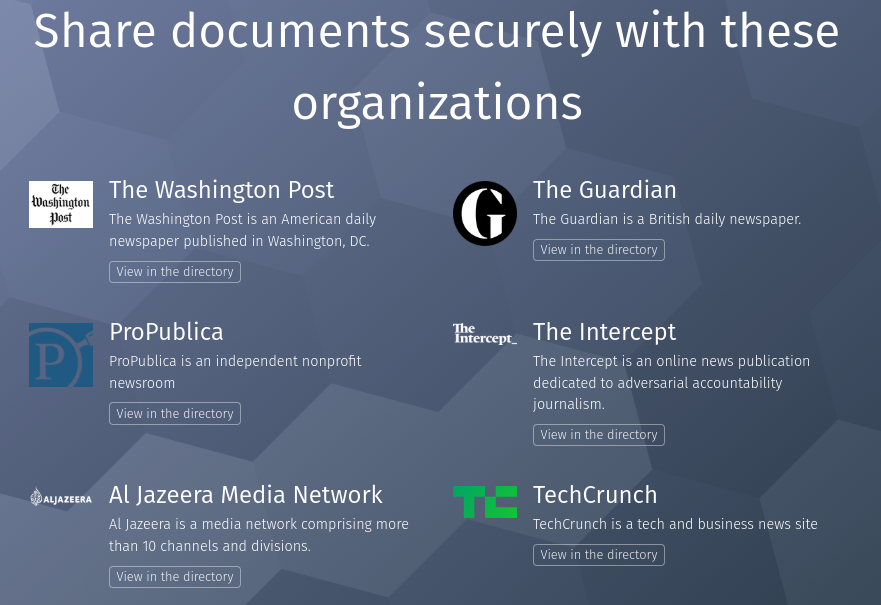
\includegraphics[width=\textwidth,height=0.4\textheight,keepaspectratio]{img/securedrop.png}

\end{frame}

%% snowden (2013)
\begin{frame}
  \frametitle{Edward Snowden (2013)}
  \framesubtitle{\url{https://theintercept.com/collections/snowden-archive/}}

  In June of 2013, a series of documents revealing the operational details
  about the Anglophone intelligence agencies' global surveillance of both
  domestic and foreign nationals.

  \pause
  \vspace{5mm}

  \begin{itemize}[<+->]
    \item Leaked by Edward Snowden, an NSA contractor to Glenn Greenwald.
    \item Led to the formation of The Intercept.
    \item Forever changed how we think about personal communication privacy.
  \end{itemize}

\end{frame}

\begin{frame}[c]
  \frametitle{Edward Snowden (2013)}
  \framesubtitle{\url{https://theintercept.com/collections/snowden-archive/}}

  \centering

  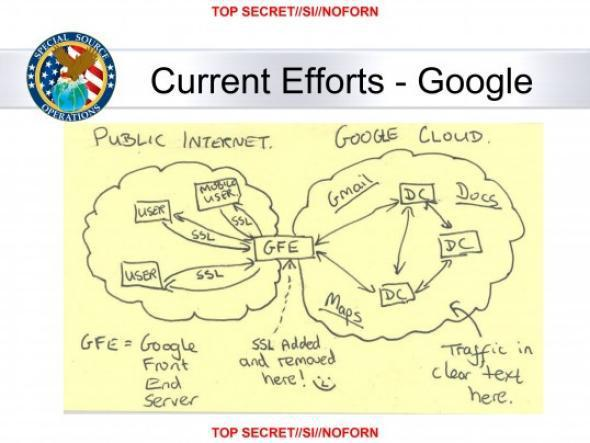
\includegraphics[width=\textwidth,height=0.6\textheight,keepaspectratio]{img/snowden_smiley.jpg}

  \emph{Slide from a Top Secret NSA presentation, explaining how they are able
  to intercept traffic from Google's users by listening in on their internal
  network past TLS termination}

\end{frame}

\begin{frame}
  \frametitle{The Internet Post-Snowden}

  SSL added and removed here :-)

  \vspace{5mm}

  \begin{columns}[c]
    \column{.45\textwidth}
    \centering
    
\includegraphics[width=.40\textwidth,height=.45\textheight,keepaspectratio]{img/logo_akamai.png}\\
    
\includegraphics[width=.40\textwidth,height=.45\textheight,keepaspectratio]{img/logo_cloudflare.jpg}
    \column{.45\textwidth}
    \centering
    
\includegraphics[width=.40\textwidth,height=.45\textheight,keepaspectratio]{img/logo_cloudfront.png}\\
    
\includegraphics[width=.40\textwidth,height=.45\textheight,keepaspectratio]{img/logo_fastly.png}\\
  \end{columns}

  \vspace{5mm}

  \centering

  \footnotesize
  \emph{Logos of Akamai, Cloudflare, Amazon Web Services Cloudfront and
  Fastly}
\end{frame}

%% spain xnet (2014)
\begin{frame}
  \frametitle{Xnet (2014)}
  \framesubtitle{\url{https://xnet-x.net/en/}}

  \begin{itemize}[<+->]
    \item Some smaller leak publishing collectives pop up around this time,
      trying to replicate the WikiLeaks model on a smaller scale, an
      interesting example being Spain's Xnet.

    \item Their biggest success was a leak from the bailed-out Bankia bank,
      whose senior executives used off-the-books Bankia credit cards to
      purchase 15 million euros worth of luxury goods, vacations and
      groceries.
  \end{itemize}

\end{frame}

%% gamma international (2014)
\begin{frame}
  \frametitle{Phineas Fisher}
  \framesubtitle{Gamma International (2014)}

  \begin{itemize}[<+->]
    \item In 2014, a new hacker persona and self-proclaimed anarchist
      revolutionary made a big splash on the scene with a hack and leak from
      German spyware company Gamma International.

    \item The person or collective, Phineas Fisher (they/them) - a
      tongue-in-cheek name after Gamma's flagship product, the FinFisher
      malware, marketed to governments and used to spy on journalists and
      dissidents.

    \item Months after the hack, Phineas Fisher released the first zine in
      the HackBack! series: \emph{HackBack!: DIY Guide for those without the
      patience to wait for whistleblowers}, giving detailed instructions aimed
      at beginner hackers on how they could reproduce the Gamma International
      hack.
  \end{itemize}

\end{frame}

\begin{frame}[c]
  \frametitle{Phineas Fisher}
  \framesubtitle{Gamma International (2014)}

  \centering
  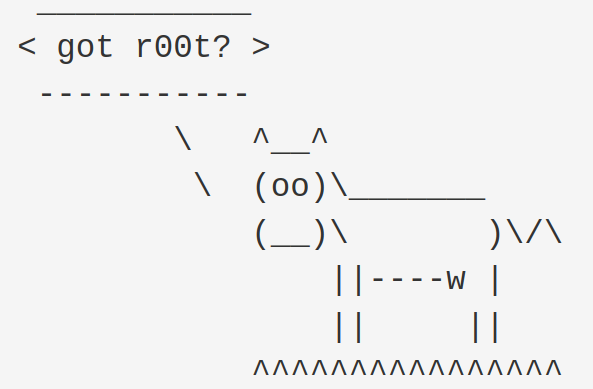
\includegraphics[width=.49\textwidth,height=.49\textheight,keepaspectratio]{img/phineas_fisher.png}
  \vspace{5mm}

  \footnotesize
  \url{https://ddosecrets.com/wiki/Finfisher}\\
  \url{https://theanarchistlibrary.org/library/phineas-fisher-hackback-a-diy-guide-ii}
\end{frame}

%% hacking team (2015)
\begin{frame}
  \frametitle{Phineas Fisher}
  \framesubtitle{Hacking Team (2015)}

  \begin{itemize}[<+->]
    \item In 2015, Phineas Fisher breached another spyware company,
      Italian cyberarms vendor Hacking Team, with WikiLeaks publishing the
      files.
    \item The company's Da Vinci and Galileo platforms allowed their customers
      to covertly compromise their target's computers and mobile phones to
      collect emails, text messages, phone call history, capture audio from
      the microphone, activate the webcam and hijack the GPS to monitor the
      target's location.
    \item The leak uncovered that HackingTeam had sold its software to
      repressive regimes with poor human rights records, including Sudan,
      Bahrain, Venezuela and Saudi Arabia.
    \item The hack was accompanied with another communique in the
      \emph{HackBack!: A DIY Guide} series.
  \end{itemize}

\end{frame}

\begin{frame}
  \frametitle{Phineas Fisher}
  \framesubtitle{Hacking Team (2015)}

  \centering
  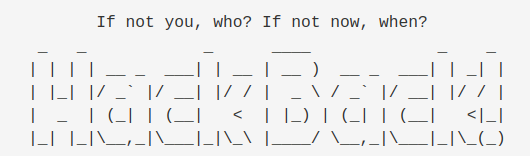
\includegraphics[width=.49\textwidth,height=.49\textheight,keepaspectratio]{img/hackback2.png}
  \vspace{1cm}

  \footnotesize
  \url{https://ddosecrets.com/wiki/Hacking_Team}\\
  \url{https://theanarchistlibrary.org/library/phineas-fisher-hackback-a-diy-guide-i}
\end{frame}

%% Football leaks (2015)
\begin{frame}
  \frametitle{Football Leaks (2015)}
  \framesubtitle{\url{https://footballleaks2015.wordpress.com/}}

  \begin{itemize}[<+->]
    \item Football Leaks was a blog set up in September 2015 revealing
      questionable financial transactions in European professional football
      and tax tricks used by the sport's biggest stars.
    \item Created by Portuguese hacker Rui Pinto.
    \item While studying in Hungary, he revealed his identity to a sports
      newspaper hoping that whistleblower protection laws would protect him
      from extradition.
    \item Unfortunately, they didn't.
    \item He was arrested in Budapest, Hungary in 2019 and was extradited at
      the request of the Portuguese authorities.
    \item Currently in house arrest, facing charges of qualified extortion,
      violation of secrecy and illegally accessing information.
  \end{itemize}

\end{frame}

\begin{frame}[c]
  \frametitle{Rui Pinto}

  \centering
  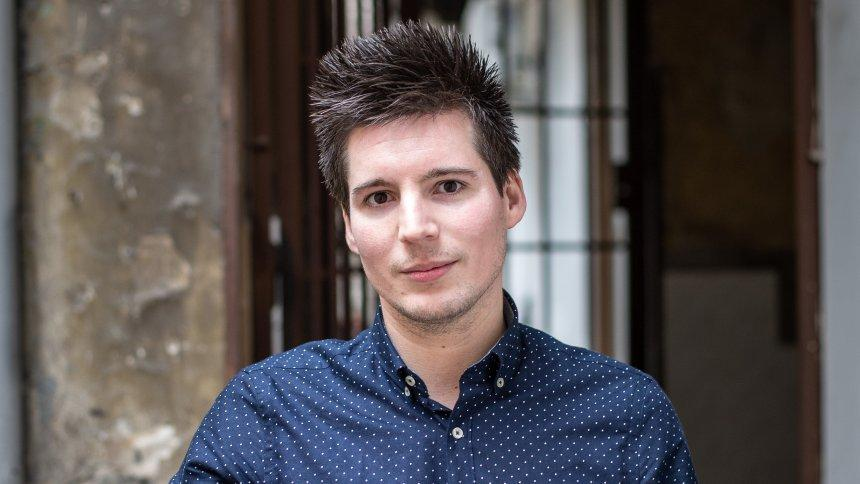
\includegraphics[width=.49\textwidth,height=.49\textheight,keepaspectratio]{img/rui_pinto.jpg}

\end{frame}

%% Panama papers (2016)
\begin{frame}
  \frametitle{Panama Papers (2016)}
  \framesubtitle{\url{https://www.icij.org/investigations/panama-papers/}}

  \begin{itemize}[<+->]
    \item A leak of 11.5 million documents (or 2.6 terabytes of data) from the
      former Panamanian offshore law firm and corporate service provider
      Mossack Fonseca.
    \item The documents contained personal financial information about wealthy
      individuals and public officials concealing money in offshore accounts,
      unraveling huge scandals all over the world.
    \item Documents leaked to the Süddeutsche Zeitung newspaper by a hacker
      calling themselves "John Doe.", later analyzed by the International
      Consortium of Investigative Journalists (ICIJ.)
    \item Led to the creation of the free software Aleph Data suite for
      searching and performing investigations on huge datasets of unstructured
      data.
    \item The full raw dataset was never made publicly available.
    \item The hacker released a manifesto, \emph{The Revolution Will Be
      Digitized}.
  \end{itemize}

\end{frame}

\begin{frame}
  \frametitle{The Revolution Will Be Digitized (excerpt)}
  \framesubtitle{John Doe}

  \begin{quote}
    Historians can easily recount how issues involving taxation and imbalances
    of power have led to revolutions in ages past. Then, military might was
    necessary to subjugate peoples, whereas now, curtailing information access
    is just as effective or more so, since the act is often invisible. Yet we
    live in a time of inexpensive, limitless digital storage and fast internet
    connections that transcend national boundaries. It doesn’t take much to
    connect the dots: from start to finish, inception to global media
    distribution, the next revolution will be digitized.

    \pause
    \vspace{3mm}
    Or perhaps it has already begun.
  \end{quote}

  \vspace{3mm}
  \centering
  \footnotesize
  \url{https://www.icij.org/investigations/panama-papers/20160506-john-doe-statement/}

\end{frame}

%% DNC leak (2016)
\begin{frame}
  \frametitle{Democratic National Committee (2016)}
  \framesubtitle{\url{https://ddosecrets.com/wiki/DNC_Emails}}

  \begin{itemize}[<+->]
    \item Leak of emails from the US Democratic Party's National Committee
      claimed by the "Guccifer 2.0" persona, now widely believed to be a cover
      used by Russian intelligence agency hackers.
    \item Released by WikiLeaks during the election race between Donald Trump
      and Hillary Clinton.
    \item Resulted in allegations of bias against Bernie Sanders' presidential
      election.
    \item The timing led people to conclude that it was a Russian operation to
      prevent Hillary Clinton from winning the election.
    \item WikiLeaks had been seemingly subverted to act as a proxy agent of
      Russian intelligence.
  \end{itemize}

\end{frame}

%% AKP Emails (2016)
\begin{frame}
  \frametitle{Phineas Fisher}
  \framesubtitle{AKP Emails (2016)}

  \begin{itemize}[<+->]
    \item In 2016, Phineas Fisher claimed responsibility for the hack of the
      Turkish ruling Justice and Development party (AKP) in solidarity with
      the Kurdish movement in Rojava and Bakur.
    \item WikiLeaks released the emails against Fisher's wishes in light of
      the attempted military coup in Turkey.
    \item \url{https://ddosecrets.com/wiki/AKP}
  \end{itemize}

\end{frame}

%% Vault 7 (2017)
\begin{frame}
  \frametitle{Vault 7 (2017)}
  \framesubtitle{\url{https://wikileaks.org/ciav7p1/}}

  \begin{itemize}[<+->]
    \item Vault 7 is a series of documents published by WikiLeaks detailing
      the activities and capabilities of the United States Central
      Intelligence Agency to perform electronic surveillance and cyber
      warfare.
    \item Detailed the agency's capabilities to hack cars, smart TVs, web
      browsers, mobile phones and personal computers.
    \item The release led to the CIA redefining WikiLeaks as a "non-state
      hostile intelligence service."
    \item In July 2022, former CIA software engineer Joshua Schulte was
      convicted of leaking the documents to WikiLeaks.
    \item The court documents from his case are very interesting:
      \url{https://archive.org/details/JoshuaSchulte}
  \end{itemize}

\end{frame}
%% Olympics doping leak (2018)
\begin{frame}
  \frametitle{Olympics Doping Leak (2018)}

  After Russia's ban from the 2018 Winter Olympics for doping
  allegations, the World Anti-Doping Agency gets hacked by Russian government
  intelligence hacker group Fancy Bear, releasing details of other nations'
  athletes prescribed performance-enhancing ADHD medication.

  \vspace{5mm}

  \centering
  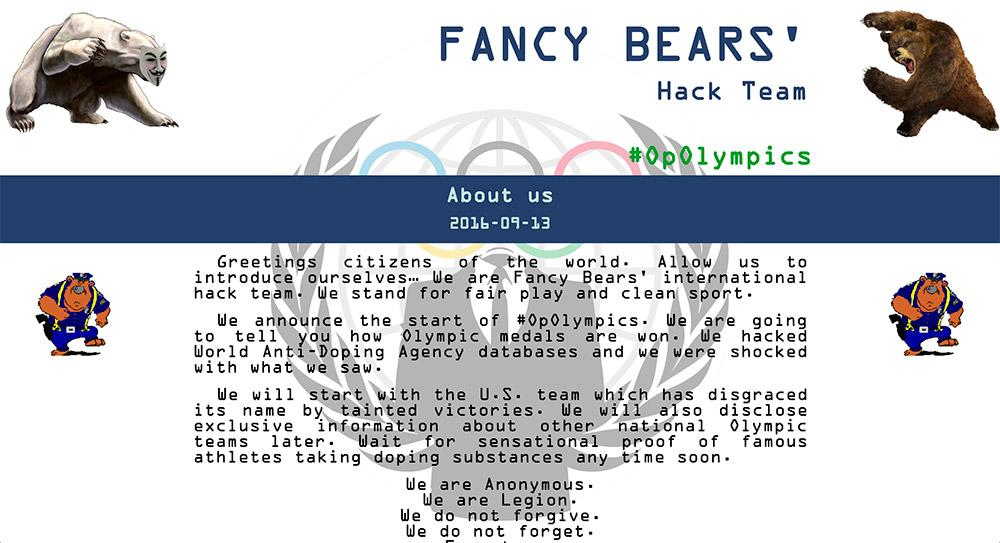
\includegraphics[width=\textwidth,height=0.5\textheight,keepaspectratio]{img/fancy_bear.jpg}

\end{frame}
%% wikileaks is dead lol
\begin{frame}[c]
  \frametitle{Assange arrested (2019)}

  \centering
  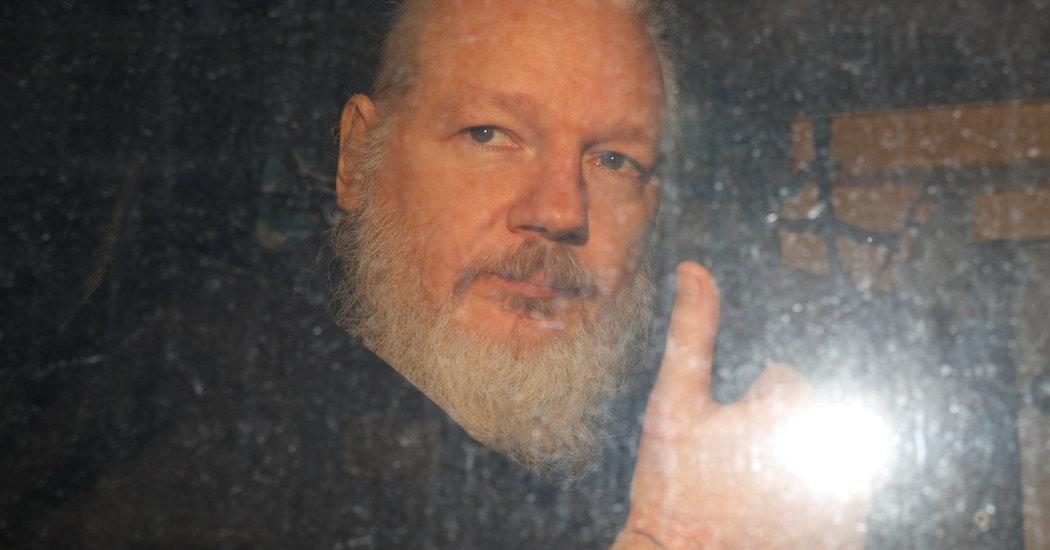
\includegraphics[width=\textwidth,height=0.5\textheight,keepaspectratio]{img/assange_arrested.jpg}

  \vspace{5mm}

  \footnotesize
  \emph{Assange giving a reporter thumbs up in the back of a British police
  van after being arrested at the Ecuadorian embassy}

\end{frame}

\begin{frame}[c]
  \frametitle{The Year is 2019}

  \begin{itemize}[<+->]
    \item Assange is arrested and placed in solitary confinement in maximum
      security Belmarsh Prison, facing extradition to the US under the
      Espionage Act.
    \item The WikiLeaks organization grows increasingly dysfunctional without
      the man at the helm, most efforts focus on fundraising for his legal
      effort.
    \item Seen as agents of Russian government.
  \end{itemize}
\end{frame}

\begin{frame}[c]
  \frametitle{The Year is 2019}

  \begin{itemize}[<+->]
    \item The DNC leak made most journalists afraid to touch data from
      hackers.
    \item Twitter bans posting any material containing data obtained from
      hacks.
    \item Growing belief every hacktivist action is a cover for foreign
      intelligence.
    \item The information security industry marketing leans on this -
      better to have their clients believe they got owned by Russian elite
      cyber soldiers than a teenager in their bedroom.
  \end{itemize}
\end{frame}

\begin{frame}[c]

  \centering

  Assange is in prison.
  \pause\hspace{1mm}WikiLeaks is dead.
  \pause\hspace{1mm}Journalists are scared to touch leaks.
  \pause\\Only Russians know how to hack.
  \pause\hspace{1mm}Hacktivism is over.
  \pause\hspace{1mm}Leaking is over.

\end{frame}

% Operation Carwash (2019)
\begin{frame}
  \frametitle{Operation Carwash (2019)}
  \framesubtitle{\url{https://theintercept.com/series/secret-brazil-archive/}}

  \begin{itemize}[<+->]
    \item On 9 June 2019, Glenn Greenwald and other journalists from The
      Intercept Brazil started publishing several messages from the
      Telegram accounts of members of the Brazilian judiciary system.
    \item Included were messages exchanged between the former Minister of
      Justice Sérgio Moro and Deltan Dellagnol, judge and prosecutor in the
      Operation Car Wash scandal that led to the arrest of former president
      Luiz Inácio Lula da Silva.
    \item The trial was accused of being politically-motivated to prevent Lula
      from running for the third term during the Bolsanaro presidency.
  \end{itemize}
\end{frame}

\begin{frame}
  \frametitle{Operation Carwash (2019)}
  \framesubtitle{\url{https://theintercept.com/series/secret-brazil-archive/}}

  \begin{itemize}[<+->]
    \item The hacker exploited a simple vulnerability in voicemail technology,
      allowing him to listen to the recorded messages for any phone number,
      unless the user has changed the default PIN code.
    \item He requested a password reset code from Telegram for the judges'
      numbers via automated phone call, which when unanswered, went to
      voicemail.
    \item Gaining access to their accounts and archived messages, he provided
      them to journalists.
    \item A simple vulnerability, helped keep Lula out of prison.
  \end{itemize}
\end{frame}

%% history section (ddosecrets era)

%% ddosecrets
\begin{frame}
  \frametitle{Distributed Denial of Secrets (2018/2019)}
  \framesubtitle{\url{https://ddosecrets.com/}}

  \centering

  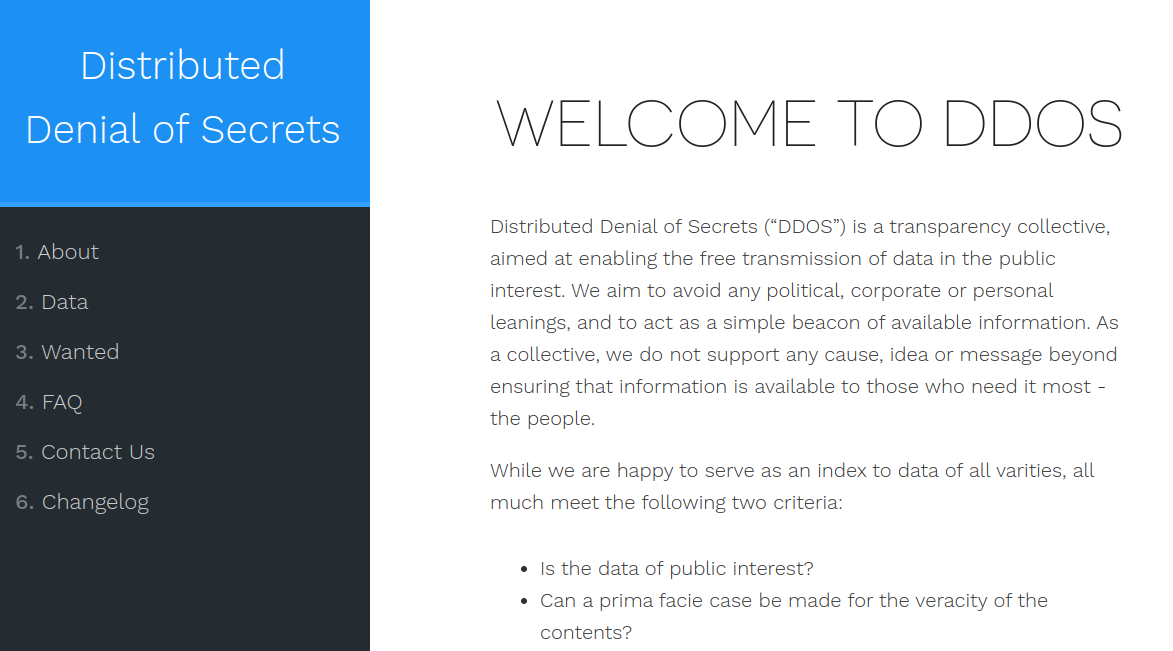
\includegraphics[width=\textwidth,height=0.6\textheight,keepaspectratio]{img/ddosecrets.png}

  \vspace{5mm}

  \footnotesize
  \emph{A screenshot of the early ddosecrets.com homepage}

\end{frame}

\begin{frame}
  \frametitle{Distributed Denial of Secrets (2018/2019)}
  \framesubtitle{\url{https://ddosecrets.com/}}

  \begin{itemize}[<+->]
    \item Founded in December 2018, by Emma Best, an online archivist and
      freedom-of-information activist based in the United States.
    \item And mysterious, anonymous figure calling themselves "the Architect."
    \item Since then, more people have joined the collective.
    \item Continue where WikiLeaks left off.
    \item Unlike WikiLeaks, only publishes raw data without editorialising the
      content.
    \item More of a leak library or archive model.
    \item Some datasets available only upon request from journalists and
      researchers.
  \end{itemize}
\end{frame}

%% Cayman National Bank and Trust (2019)
\begin{frame}
  \frametitle{Phineas Fisher}
  \framesubtitle{Cayman National Bank and Trust (2019)}

  \begin{itemize}[<+->]
    \item The Phineas Fisher hacktivist persona makes an unexpected comeback
      with a hack, leak and robbery of the Cayman National Bank and Trust in
      the Isle of Man.
    \item Phineas Fisher provided a complete copy of the bank's servers to
      Distributed Denial of Secrets, investigated by Unicorn Riot, Global
      Witness and Organized Crime and Corruption Reporting Project.
    \item Isle of Man had a growing reputation as a tax haven for private jet
      purchases in Europe.
    \item Published another entry in the HackBack! series, \emph{HackBack!: A
      DIY guide to robbing banks}, detailing the bank robbery from start to
      finish.
    \item Donated part of the money to the Rojava revolutionary project, and
      offered a "Hacktivist Bug Bounty" of up to \$100,000 for similar
      politically motivated hacks and leaks.
  \end{itemize}

\end{frame}

\begin{frame}[c]
  \frametitle{Phineas Fisher}
  \framesubtitle{Cayman National Bank and Trust (2019)}

  \begin{quote}
    I hacked a bank. I did it to give an injection of liquidity, but this time
    from below, for the simple and humble people that resist and rebel against
    injustice all over the world. In other words, I robbed a bank and gave
    away the money.
  \end{quote}

\end{frame}

\begin{frame}[c]
  \frametitle{Phineas Fisher}
  \framesubtitle{Cayman National Bank and Trust (2019)}

  \centering
  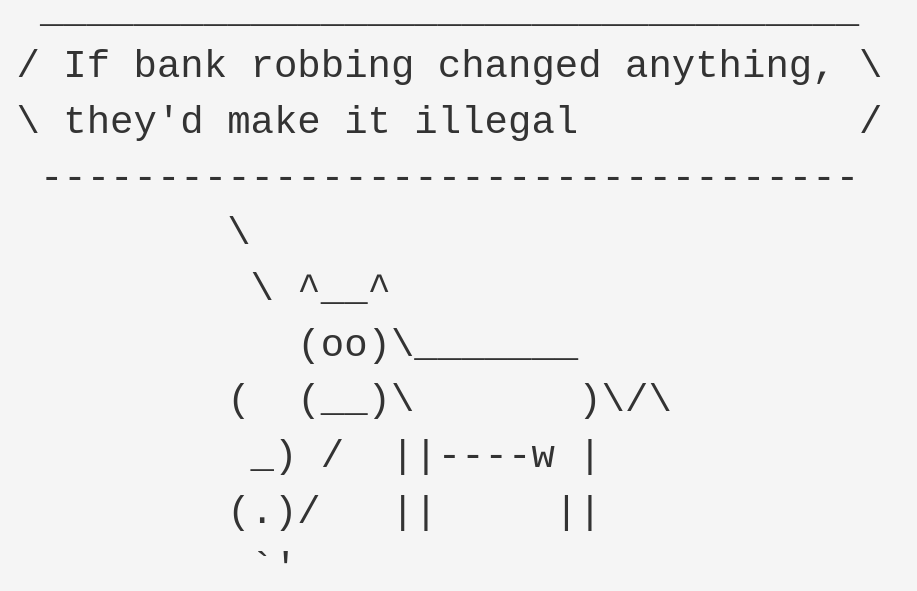
\includegraphics[width=\textwidth,height=0.4\textheight,keepaspectratio]{img/hackback_sherwood.png}

  \vspace{5mm}

  \footnotesize
  \url{https://ddosecrets.com/wiki/Sherwood}\\
  \url{https://theanarchistlibrary.org/library/subcowmandante-marcos-hack-back}

\end{frame}

%% Paco Leaks (2019)
%% Milico Leaks (2019)
\begin{frame}
  \frametitle{PacoLeaks and MilicoLeaks (2019)}
  \framesubtitle{\url{https://ddosecrets.com/wiki/PacoLeaks} \url{https://ddosecrets.com/wiki/MilicoLeaks}}

  \begin{itemize}[<+->]
    \item PacoLeaks, thousands of files taken from the Chilean National
      Police.
    \item MilicoLeaks, leaks of email from senior officials and officers in
      the Chilean army.
    \item Data published by Distributed Denial of Secrets.
    \item Investigation by CIPER, confirmed suspected fraud related to travel
      expenses, a biliteral intelligence sharing agreement between Chilean
      military and the US and trips to Israel for military commanders to
      attend cybersecurity trainings.
    \item Phineas Fisher paid their first "Hacktivist Bug Bounty" to
      Matapacos, the hacktivist behind MilicoLeaks.
  \end{itemize}
\end{frame}

\begin{frame}[c]
  \frametitle{Matapacos}

  \centering

  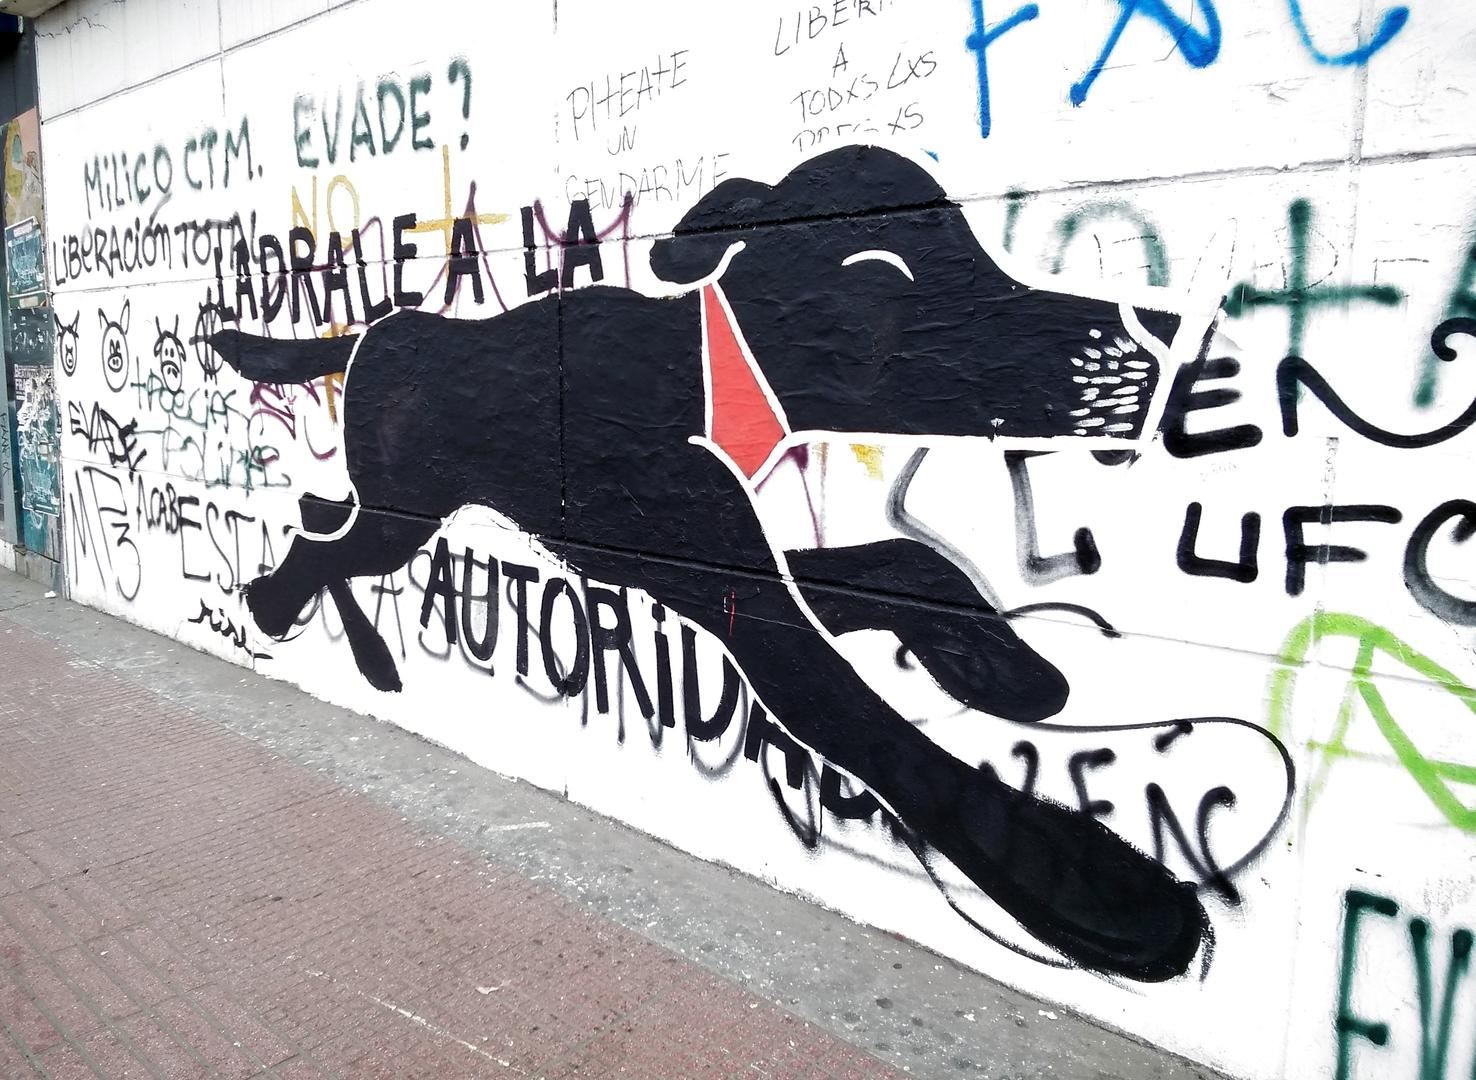
\includegraphics[width=\textwidth,height=0.7\textheight,keepaspectratio]{img/matapacos.jpg}

  \footnotesize
  \emph{Negro Matapacos (Black Cop-Killer) was a Chilean stray dog who
  acquired fame due to his participation in the Santiago 2011 street protests
  (Photo: Sfs90, Wikimedia Commons)}

\end{frame}

%% Luanda Leaks (2020)
\begin{frame}
  \frametitle{Luanda Leaks (2020)}
  \framesubtitle{\url{https://www.icij.org/investigations/luanda-leaks/}}

  \begin{itemize}[<+->]
    \item In January 2020, the ICIJ published a report on how Isabel dos
      Santos, the daughter of Angola's former president José Eduardo dos
      Santos, once considered Africa's richest woman, amassed her wealth.
    \item Three days after the leak, her personal wealth manager was found
      dead in the garage of his house.
  \end{itemize}
\end{frame}

\begin{frame}
  \frametitle{Luanda Leaks (2020)}
  \framesubtitle{\url{https://www.icij.org/investigations/luanda-leaks/}}

  \begin{itemize}[<+->]
    \item Leak claimed by Portuguese hacker Rui Pinto.
    \item Caused controversy and raised more ethical questions over working
      with hacked data as Rui allegedly attempted to extort dos Santos not to
      leak the data.
    \item Some people actually believed Rui Pinto ruined leaking forever and
      nobody would ever want to touch hacked data ever again after this.
    \item Bad for his criminal case, spoiled his claims of being an ethical
      whistleblower.
    \item Still being reported on in 2023 despite this.
  \end{itemize}

\end{frame}
%% BlueLeaks (2020)
\begin{frame}
  \frametitle{BlueLeaks (2020)}
  \framesubtitle{\url{https://ddosecrets.com/wiki/BlueLeaks}}

  \begin{itemize}[<+->]
    \item Leak of 269.21 gigabytes of internal U.S. law enforcement data
      obtained by the hacker collective Anonymous.
    \item Released on June 19, 2020 in support of the Black Lives Matter
      movement and George Floyd protests.
    \item Published by Distributed Denial of Secrets.
    \item Data originated from breach of security breach of Netsential, a
      web developer that works with fusion centers and law enforcement. Comes
      largely from intelligence gathered from fusion centers.
    \item Fusion centers, set up to improve communication between different
      levels of law enforcement, have been critized as privacy-invading,
      ineffective and targeted at political groups.
  \end{itemize}

\end{frame}

\begin{frame}
  \frametitle{BlueLeaks (2020)}
  \framesubtitle{\url{https://ddosecrets.com/wiki/BlueLeaks}}

  \begin{itemize}[<+->]
    \item Heavily suppressed by law enforcement from social media coverage.
    \item Mainstream media afraid to cover it due to the lasting stigma around
      hacked data from the WikiLeaks era.
    \item (It must had been the Russians)
    \item Twitter shadowbans the \texttt{\#blueleaks} hashtag.
    \item Twitter bans the official Distributed Denial of Secrets
      \texttt{@ddosecrets} account under the distribution of hacked materials
      policy.
    \item Reddit bans the \texttt{/r/blueleaks} subreddit.
    \item You cannot link to \url{https://ddosecrets.com/} on Twitter to
      this day.
  \end{itemize}

\end{frame}

\begin{frame}
  \frametitle{BlueLeaks (2020)}
  \framesubtitle{\url{https://ddosecrets.com/wiki/BlueLeaks}}

  \begin{itemize}[<+->]
    \item Distributed Denial of Secrets gets the server hosting their Aleph
      search engine \texttt{hunter.ddosecrets.com} seized in Germany under
      a mutual legal aid request from the United States.
    \item Administrators of sites mirroring the data, like The Eye get visits
      from Immigration and Customs Enforcement (ICE.)
    \item Ongoing federal law enforcement investigation.
  \end{itemize}

\end{frame}

\begin{frame}
  \frametitle{BlueLeaks (2020)}
  \framesubtitle{\url{https://ddosecrets.com/wiki/BlueLeaks}}

  \begin{itemize}[<+->]
    \item Contains over one million documents, internal memos,
      financial records, and more from over 200 state, local and federal
      agencies.
    \item In the leaked documents, officers track individual, group, and event
      pages with protest or anti-law enforcement rhetoric.
    \item Some of the documents related to the law enforcement response to the
      Black Lives Matter movement and George Floyd protests.
    \item Including monitoring of the protesters' communications over social
      media and messaging apps.
    \item Much of the data still unexplored and waiting to be investigated.
  \end{itemize}

\end{frame}

\begin{frame}[c]
  \frametitle{BlueLeaks (2020)}
  \framesubtitle{\url{https://ddosecrets.com/wiki/BlueLeaks}}

  \centering

  \scriptsize

  \url{magnet:?xt=urn:btih:8cf92b7cd3f022fa5478b84963e89c1dd0af090f&dn=BlueLeaks&tr=udp\%3A\%2F\%2Ftracker.coppersurfer.tk\%3A6969\%2Fannounce&tr=udp\%3A\%2F\%2F9.rarbg.to\%3A2920\%2Fannounce&tr=udp\%3A\%2F\%2Ftracker.opentrackr.org\%3A1337&tr=udp\%3A\%2F\%2Ftracker.leechers-paradise.org\%3A6969\%2Fannounce&tr=udp\%3A\%2F\%2Ftracker.coppersurfer.tk\%3A6969\%2Fannounce}

  
\includegraphics[width=0.25\textwidth,height=0.25\textwidth,keepaspectratio]{img/blueleaks_qr.png}

  \normalsize

  \url{ipfs:QmdUQ2d2PGA5q1L4pDhd9fek1ejzowbZKTMCnAYR2EgViA}

\end{frame}

%% Parler (2021)
\begin{frame}
  \frametitle{Parler (2021)}
  \framesubtitle{\url{https://ddosecrets.com/wiki/Parler}}

  \begin{itemize}[<+->]
    \item On 6th of January, during the certification of U.S. election results
      in which Donald Trump lost to Joe Biden, a group of Trump supporters
      storm the U.S. Capitol in an attempt to overthrow the government.
    \item Twitter bans Donald Trump's Twitter account to prevent further
      violence.
    \item Much of the planning of and the attack itself was captured live by
      the attackers themselves on alternative fascist social media sites
      Parler and Gab.
  \end{itemize}
\end{frame}

\begin{frame}
  \frametitle{Parler (2021)}
  \framesubtitle{\url{https://ddosecrets.com/wiki/Parler}}

  \begin{itemize}[<+->]
    \item Google and Apple announce that they will be removing Parler from
      their respective app stores.
    \item Amazon Web Services announces that they will no longer be providing
      hosting services to Parler, with 48 hours notice.
    \item One hacker, donk\_enby realizes that with Parler gone, so would be
      the historical record of an important event in US history and a wealth
      of criminal evidence against the attackers.
  \end{itemize}

\end{frame}

\begin{frame}
  \frametitle{Parler (2021)}
  \framesubtitle{\url{https://ddosecrets.com/wiki/Parler}}

  \begin{itemize}[<+->]
    \item Using previous research into Parler's inner workings, donk is
      able to enumerate every video and picture ever posted to Parler and
      every post made during the attack.
    \item Via Twitter, organizes a grassroot effort to crowdsource the
      bandwidth and storage to save all content from Parler before Amazon AWS
      shuts it down.
    \item Posts get preserved in Internet Archive's Wayback Machine (53.71TB)
    \item A cache of over a million video files (32.1TB) and 235GB image files
      gets shared with Distributed Denial of Secrets.
    \item Donk is able to exploit a flaw in Parler's video upload system
      to get the original files uploaded by the users before transcoding and
      stripping of metadata.
    \item The metadata in the original video files contain embedded GPS
      coordinates and timestamps of when and where the videos were taken.
  \end{itemize}

\end{frame}

\begin{frame}[c]
  \frametitle{Parler (2021)}
  \framesubtitle{\url{https://www.adambreuer.com/map}}

  This allows people to very quickly sort through the millions of videos
  and narrow down the dataset to the ones taken during and at the attack
  on the Capitol.

  \vspace{3mm}

  \centering
  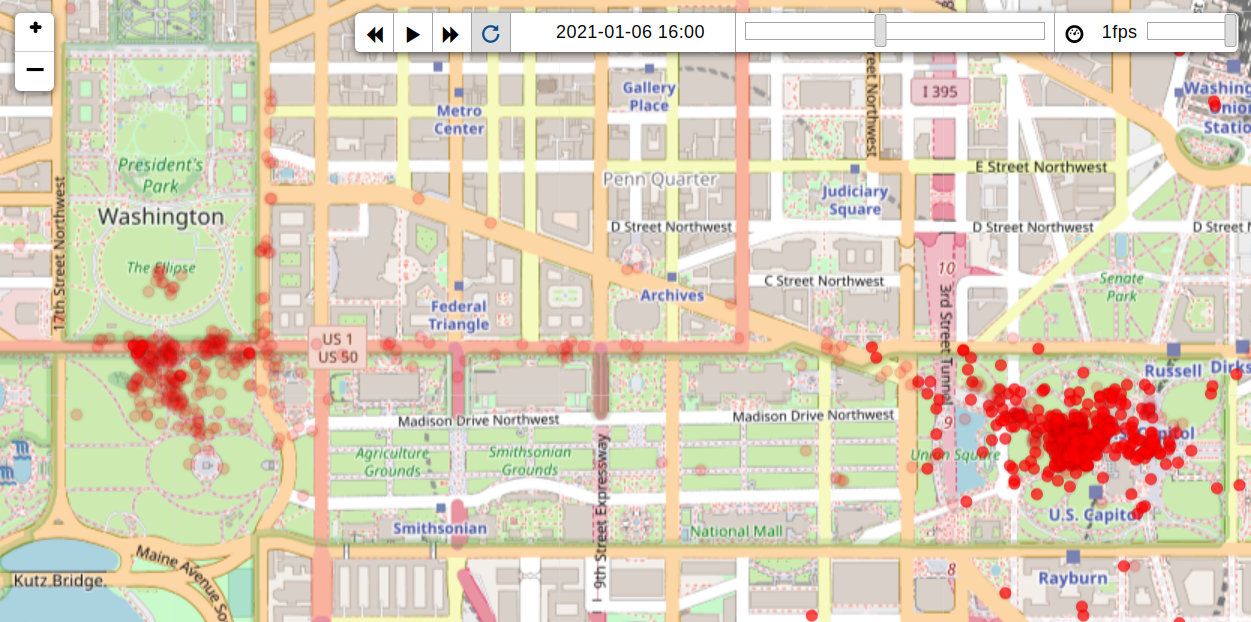
\includegraphics[width=\textwidth,height=0.4\textheight,keepaspectratio]{img/parler_map.png}

  \vspace{2mm}
  \footnotesize
  \emph{Interactive timeline of videos from the attack}

\end{frame}

\begin{frame}
  \frametitle{Parler (2021)}
  \framesubtitle{\url{https://projects.propublica.org/parler-capitol-videos/}}

  \footnotesize
  ProPublica publishes an interactive video timeline of the attack within two
  weeks of the data being released.

  \centering \vfill
  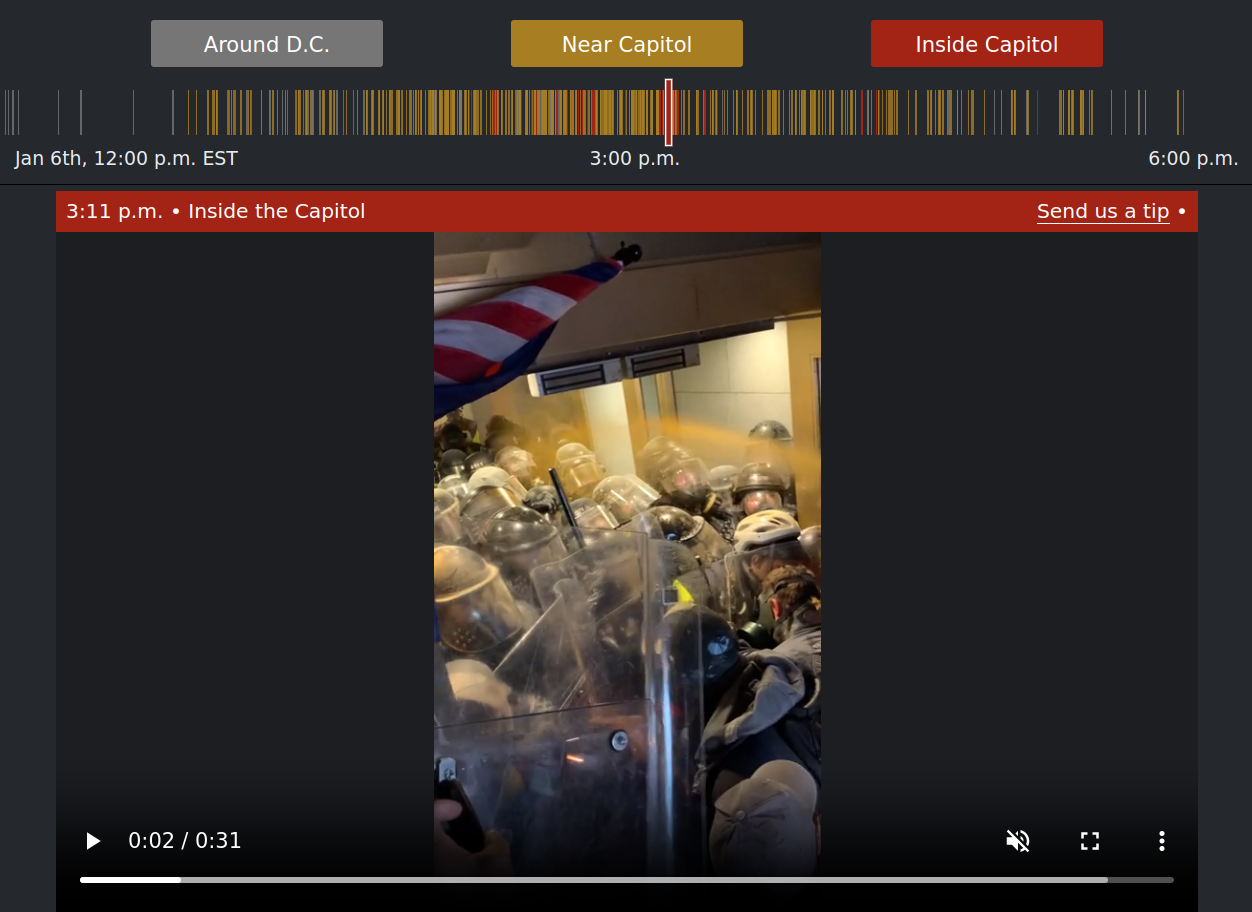
\includegraphics[width=\textwidth,height=0.6\textheight,keepaspectratio]{img/parler_propublica.png}

  \emph{What Parler Saw During the Attack on the Capitol (ProPublica, 17th
  January 2021)}

\end{frame}

\begin{frame}
  \frametitle{Parler (2021)}
  \framesubtitle{\url{https://ddosecrets.com/wiki/Parler}}

  \footnotesize
  Videos from Parler make up the bulk of evidence against Donald Trump in
  his second impeachment case, sourced from the ProPublica timeline.

  \centering \vfill
  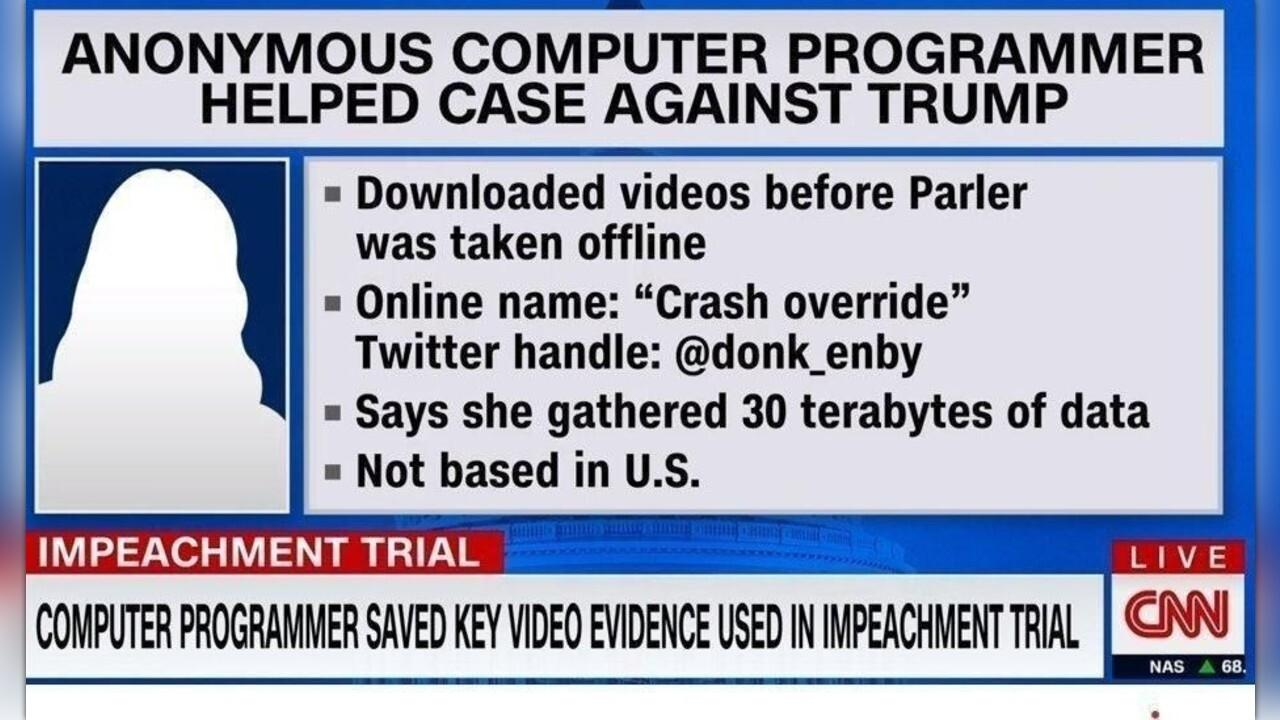
\includegraphics[width=\textwidth,height=0.6\textheight,keepaspectratio]{img/parler_cnn.png}

  \emph{Screencap from a CNN news report: Anonymous Computer Programmer Helps
  Case Against Trump}

\end{frame}

\begin{frame}
  \frametitle{Parler (2021)}
  \framesubtitle{\url{https://ddosecrets.com/wiki/Parler}}

  \begin{itemize}[<+->]
    \item Videos and posts from Parler make a frequent appearance in criminal
      proceedings against the Capitol rioters.
    \item 982 suspects indicted, charged or sentenced to date.
    \item \url{https://seditiontracker.com/suspects/by_name}
  \end{itemize}

\end{frame}

\begin{frame}[fragile]
  \frametitle{Parler (2021)}
  \framesubtitle{Parler Tricks}

  \begin{lstlisting}[language=Python,basicstyle=\scriptsize,commentstyle=\color{Brown}]
  def reverse_convert(self, _type, _id):
  '''
  GET /v3/uuidConversion/{type}/{id}
  (*) this is enumerable
  params:
  type: one of (user, post, comment, image, video, link)
  id: hidden, sequential ID
  response:
  public-facing UUID of the entity
  rate-limit: none
  auth: yes
  '''
  return self.s.get(
  "{}/v3/uuidConversion/{}/{}".format(self.root_url, _type, _id)
  )
  \end{lstlisting}

  \centering
  \footnotesize
  \url{https://github.com/d0nk/parler-tricks}

\end{frame}

\begin{frame}
  \frametitle{Parler (2021)}
  \framesubtitle{\url{https://ddosecrets.com/wiki/Parler}}

  \begin{itemize}
    \item
      \href{https://gizmodo.com/every-deleted-parler-post-many-with-users-location-dat-1846032466}{\textcolor{blue}{Every
      Deleted Parler Post, Many With Users' Location Data, Has Been Archived}
      - Gizmodo}
    \item
      \href{https://www.vice.com/en/article/n7vqew/the-hacker-who-archived-parler-explains-how-she-did-it-and-what-comes-next}{\textcolor{blue}{The
      Hacker Who Archived Parler Explains How She Did It}} - Vice
    \item \href{https://arxiv.org/pdf/2101.03820.pdf}{\textcolor{blue}{An
      Early Look at the Parler Online Social Network}} - NYU Cyber Lab - Max
      Aliapoulios, Emmi Bevensee, Jeremy Blackburn, Barry Bradlyn, Emiliano De
      Cristofaro, Gianluca Stringhini and Savvas Zannettou
    \item
      \href{https://stacks.stanford.edu/file/druid:gw857tq5527/20210128-parler.pdf}{\textcolor{blue}{Contours
      and Controversies of Parler}} - Stanford Internet Observatory - Thiel,
      D., DiResta, R., Grossman, S., and Cryst, E. (2021)
  \end{itemize}

\end{frame}

\begin{frame}[c]
  \frametitle{Parler (2021)}
  \framesubtitle{\url{https://ddosecrets.com/wiki/Parler}}

  \begin{quote}
    Everything we grabbed was publicly available on the web, we just made a
    permanent public snapshot of it.
  \end{quote}

  \vspace{5mm}
  \centering
  \footnotesize
  \url{https://www.vice.com/en/article/5dpkvx/every-video-ever-posted-to-parler-is-now-available-to-download}

\end{frame}

%% Myanmar Investments (2021)
\begin{frame}
  \frametitle{Myanmar Financials (2021)}
  \framesubtitle{\url{https://ddosecrets.com/wiki/Myanmar_Financials}}

  \begin{itemize}[<+->]
    \item After the military coup overthrowing the democratically government
      in Myanmar, people started reaching out to hackers like Donk asking for
      help on Twitter.
    \item Donk focused on scraping any publicly available financial
      information that might expose cronyism of the leaders of the
      junta, data at risk of disappearing from the Internet after the coup.
    \item Released the 330.5GB Myanmar Financials dataset includes corporate
      registry information, incorporation documents of 120k companies,
      beneficial ownership disclosures for the gem and mining industry and
      public tenders
    \item Published via Distributed Denial of Secrets.
  \end{itemize}

\end{frame}

\begin{frame}
  \frametitle{Myanmar Investments (2021)}
  \framesubtitle{\url{https://ddosecrets.com/wiki/Myanmar_Investments}}

  \begin{itemize}[<+->]
    \item The hackers were also able to gain privileged access to the
      government's investment portal and leak details (156GB) of foreign
      investments in the mining, hotel and petroleum industry, now
      funding the military junta.
    \item The military junta who was now shooting peaceful protesters in
      the streets.
    \item The data gets investigated in conjunction with a covert group of
      Myanmar activists, Justice for Myanmar.
  \end{itemize}
\end{frame}

\begin{frame}
  \frametitle{Myanmar Investments (2021)}
  \framesubtitle{\url{https://ddosecrets.com/wiki/Myanmar_Investments}}
  \begin{itemize}[<+->]
    \item Causes a huge scandal in France, with Le Monde running a front-page
      story based on the leak about Total's involvement in funding the coup.
    \item Total pulls all advertisement from Le Monde in anger.
    \item Then change their minds and hold an emergency meeting with
      shareholders to apologize.
    \item Total and Chevron decide to end their operations in Myanmar by
      the end of the year as a result of the leak.
  \end{itemize}
\end{frame}

\begin{frame}
  \frametitle{Myanmar Investments (2021)}
  \framesubtitle{\url{https://ddosecrets.com/wiki/Myanmar_Investments}}

  The source, working under the nom-de-guerre "Sugondese separatist Bofa"
  released a statement detailing the technical details and their motivations
  for the leak

  \vspace{1mm}

  \centering
  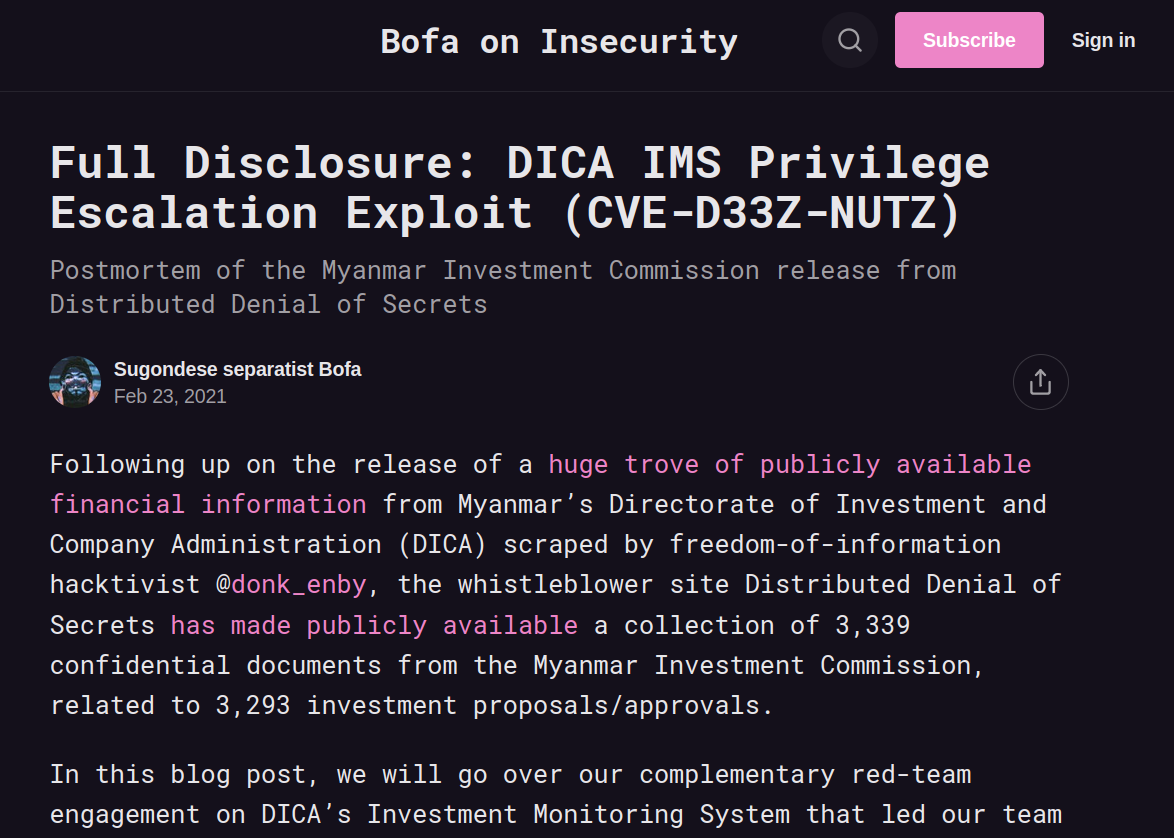
\includegraphics[width=\textwidth,height=0.55\textheight,keepaspectratio]{img/myanmar_investments.png}

  \footnotesize
  \url{https://bofa.substack.com/p/full-disclosure-dica-ims-privilege}

\end{frame}

% gab
\begin{frame}
  \frametitle{Gab (2021)}
  \framesubtitle{\url{https://ddosecrets.com/wiki/GabLeaks}}

  \begin{itemize}[<+->]
    \item Gab was another fascist social media site, similar to Parler.
    \item Open-source codebase based on Mastodon, SQL injection vulnerability
      introduced by the company's Chief Technology Officer.
    \item Exploited to obtain every post ever made on Gab, as well as every
      private post and private message.
    \item Leaked to Distributed Denial of Secrets by hacktivist JaXpArO
      (they/them) \& My Little Anonymous Revival Project.
    \item Limited distribution as the dataset includes private messages of
      users doxxing leftist and anti-fascist political activists.
    \item In response, Gab CEO Andrew Torba makes a public post referring to
      Distributed Denial of Secrets as a group of "mentally ill [t-slur] demon
      hackers."
  \end{itemize}
\end{frame}

% verkada

\begin{frame}
  \frametitle{Verkada (2021)}
  \framesubtitle{\url{https://en.wikipedia.org/wiki/Maia_arson_crimew}}

  \begin{itemize}[<+->]
    \item In March 2011, Swiss hacktivist maia arson crimew gets indicted by a grand
      jury in the United States shortly after her hack of the Verkada video
      surveillance vendor, for an alleged hacking spree spanning three years
      motivated by her opposition to intellectual property.
    \item crimew's home was raided and her devices seized.
    \item Switzerland does not extradite its own citizens.
    \item The seized devices have since been returned as Switzerland does not
      turn over evidence to foreign countries in cases of alleged political
      activism.
  \end{itemize}

\end{frame}

\begin{frame}
  \frametitle{Verkada (2021)}
  \framesubtitle{\url{https://en.wikipedia.org/wiki/Maia_arson_crimew}}

  \centering
  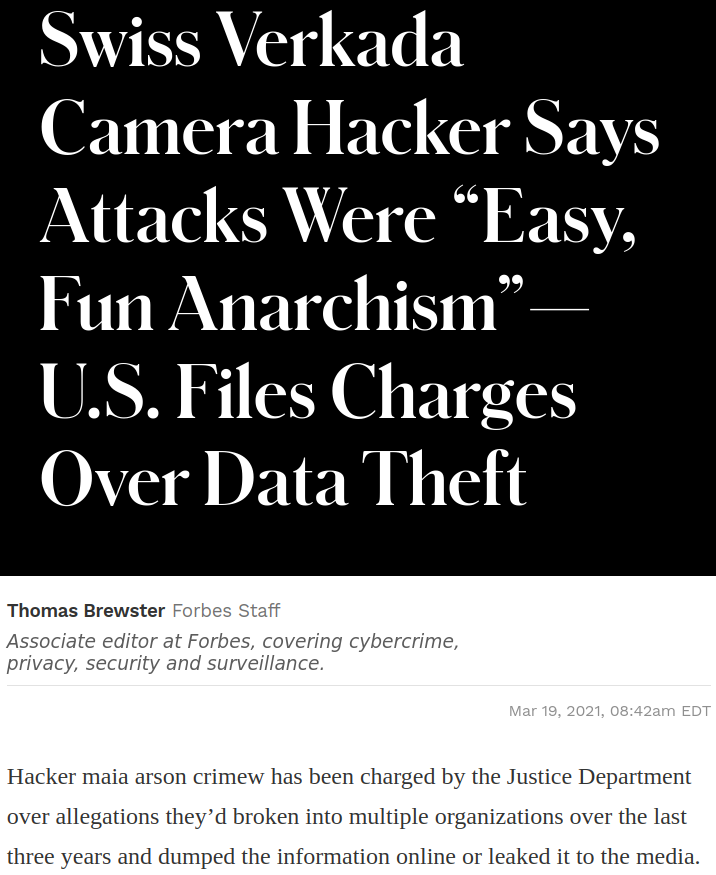
\includegraphics[width=\textwidth,height=0.7\textheight,keepaspectratio]{img/verkada_forbes.png}

  \footnotesize
  \emph{Forbes - Swiss Verkada Camera Hacker Says Attacks Were "Easy, Fun
  Anarchism" - U.S. Files Charges Over Data Theft}

\end{frame}

\begin{frame}[c]
  \frametitle{maia arson crimew}
  \framesubtitle{\url{https://en.wikipedia.org/wiki/Maia_arson_crimew}}

  \centering
  
\includegraphics[width=\textwidth,height=0.7\textheight,keepaspectratio]{img/maia_arson_crimew.jpg}

  \footnotesize
  \emph{A selfie of crimew in 2022, CC BY-SA, maia arson crimew}

\end{frame}

\begin{frame}[c]

  \begin{quote}
    Another one got caught today, it's all over the papers.
    "Teenager Arrested in Computer Crime Scandal", "Hacker Arrested after Bank
    Tampering"...\\Damn kids. They're all alike.
  \end{quote}

  \vspace{5mm}

  \centering
  \footnotesize
  \emph{\href{https://en.wikisource.org/wiki/The_Hacker_Manifesto}{\textcolor{blue}{The Hacker Manifesto - Loyd Blankenship}}}

\end{frame}

%% Tea Party Patriots (2021) / America's Frontline Doctors (2021)
\begin{frame}[c]
  \frametitle{Tea Party Patriots (2021)}
  \framesubtitle{\url{https://theintercept.com/2021/08/05/tea-party-patriots-hacked-billionaire-donors/}}

  \centering
  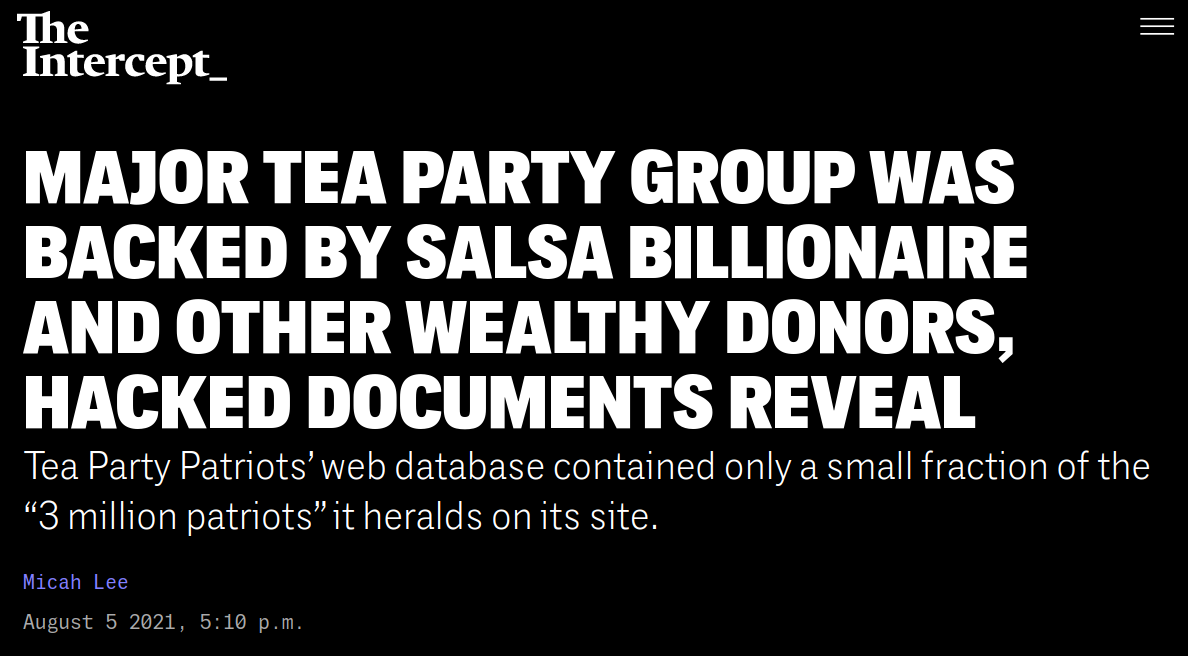
\includegraphics[width=\textwidth,height=0.7\textheight,keepaspectratio]{img/tea_party_patriots.png}

  \footnotesize
  \emph{The Intercept - Major Tea Party Group Was Backed By Salsa Billionaire
  and Other Wealthy Donors, Hacked Documents Reveal}

\end{frame}

\begin{frame}[c]
  \frametitle{America's Frontline Doctors (2021)}
  \framesubtitle{\url{https://theintercept.com/2021/09/28/covid-telehealth-hydroxychloroquine-ivermectin-hacked/}}

  \centering
  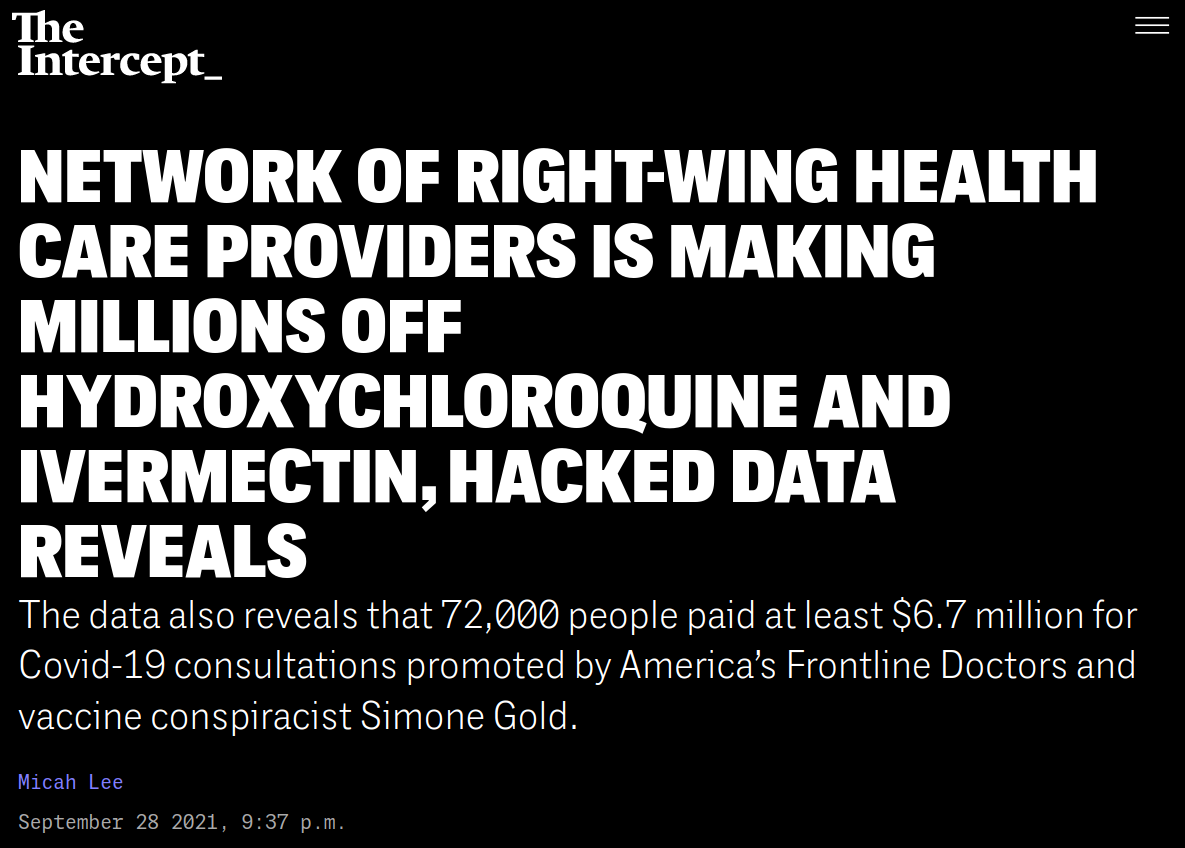
\includegraphics[width=\textwidth,height=0.7\textheight,keepaspectratio]{img/americas_frontline_doctors.png}

  \footnotesize
  \emph{The Intercept - Network of Right-Wing Health Care Providers is Making
  Millions Off Hydroxychloroquine and Ivermectin, Hacked Data Reveals}

\end{frame}

%% Twitch (2021)
\begin{frame}
  \frametitle{TwitchLeaks (2021)}
  \framesubtitle{\url{https://ddosecrets.com/wiki/Twitch}}

  \centering
  \movie[width=\textwidth,height=0.75\textheight]{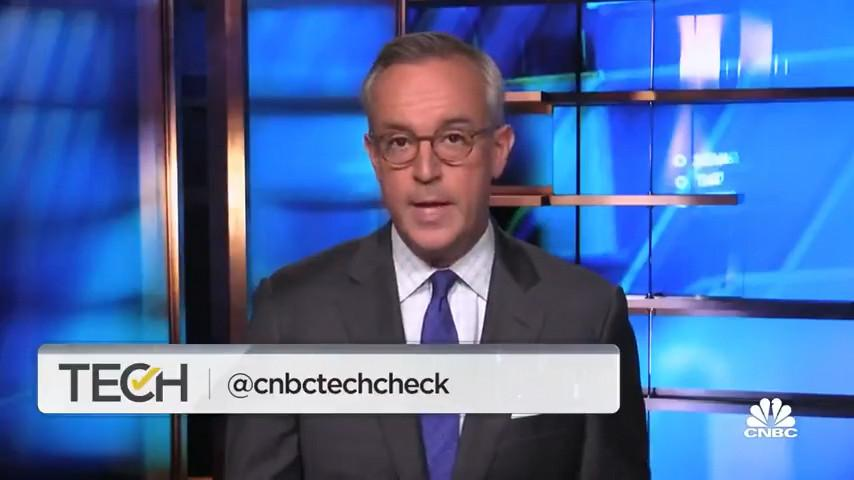
\includegraphics[width=\textwidth,height=0.75\textheight]{img/twitch.jpg}}{img/twitch.mp4}

  \footnotesize
  \emph{CNBC Tech Check - Twitch hacked}
\end{frame}

\begin{frame}
  \frametitle{TwitchLeaks (2021)}
  \framesubtitle{\url{https://ddosecrets.com/wiki/Twitch}}

  \footnotesize

  The leak included Twitch's entire source code base and exposed the real
  payouts of the platform's biggest stars. But also:\pause

  \vfill \centering
  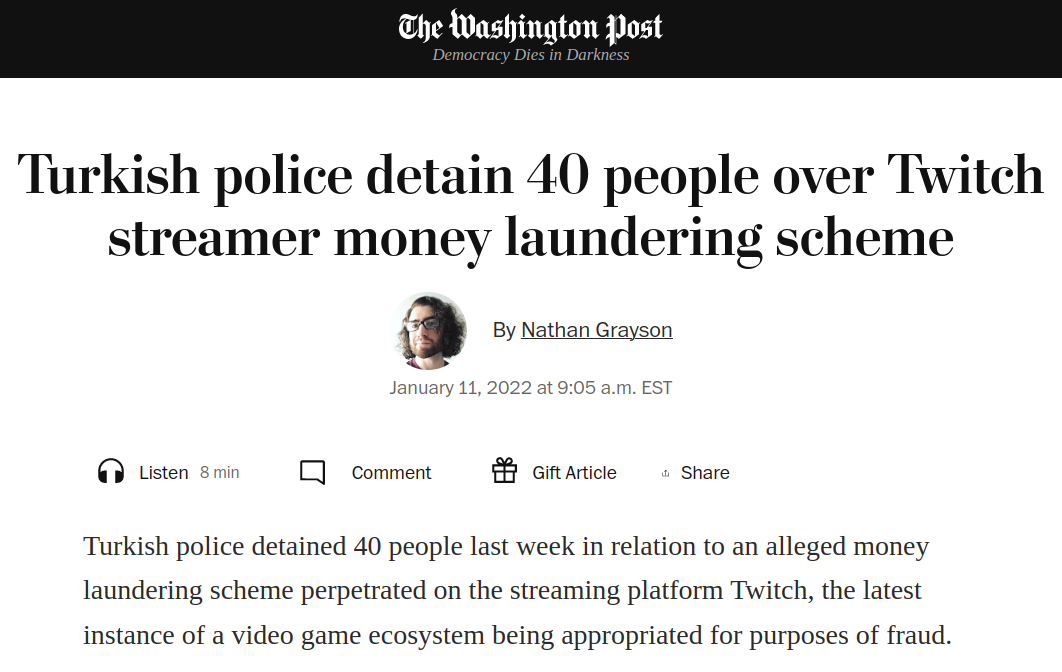
\includegraphics[width=\textwidth,height=0.6\textheight,keepaspectratio]{img/twitch_leaks_turkey.png}

  \url{https://www.washingtonpost.com/video-games/2022/01/11/twitch-bit-money-laundering-turkey-police/}
\end{frame}

%% Metropolitan Police Department D.C. (2021)
\begin{frame}
  \frametitle{Metropolitan Police Department, D.C (2021)}
  \framesubtitle{\url{https://ddosecrets.com/wiki/Metropolitan_Police_Department_D.C.}}

  \begin{itemize}[<+->]
    \item A leak of the Metropolitan Police D.C. police containing a 156.35 GB
      "gang database," emails and human resources data.
    \item Interesting because the leak came as a result of a hack by the
      ransomware group Babuk - it was financially, not politically motivated.
    \item The hackers encrypted one of the computer's on the police
      department's network, then tried to extort them for money not to leak
      confidential information from the department's network.
    \item The police did not pay and the hackers leaked the data.
  \end{itemize}
\end{frame}

\begin{frame}
  \frametitle{Metropolitan Police Department, D.C (2021)}
  \framesubtitle{\url{https://ddosecrets.com/wiki/Metropolitan_Police_Department_D.C.}}

  \begin{itemize}[<+->]
    \item Distributed Denial of Secrets mirrored it and provided it to
      journalists.
    \item The emails revealed amongst other things that the police department
      tried to suppress robberies by stopping and frisking and surveiling
      residents of black neighborhoods.
    \item
      \url{https://theappeal.org/dc-police-robbery-crackdown-leaked-emails/}
  \end{itemize}
\end{frame}

\begin{frame}[c]
  \frametitle{Metropolitan Police Department, D.C (2021)}
  \framesubtitle{\url{https://emma.best/2021/05/13/metropolitan-police-department-d-c-ransomware-negotiations/}}

  \small

  \textbf{Babuk, May 9, 1:05 PM}: \texttt{Any updates?}

  \vspace{3mm} \pause

  \textbf{MPD, May 10, 3:51 PM}: \texttt{shortly}

  \vspace{3mm} \pause

  \textbf{MPD, May 10, 4:57 PM}: \texttt{Our final proposal is an offer to pay
  \$10,000 to prevent the release of the stolen data. If this offer is not
  acceptable, then it seems our conversation is complete. I think we both
  understand the consequences of not reaching an agreement. We are OK with
  that outcome.}

  \vspace{3mm} \pause

  \textbf{Babuk, May 10, 5:08 PM}: \texttt{This is unacceptable from our side.
  Follow our web-site at midnight.}

\end{frame}

%% GiveSendGo (2021/2022)
\begin{frame}
  \frametitle{GiveSendGo (2021/2022)}
  \framesubtitle{\url{https://ddosecrets.com/wiki/GiveSendGo}}

  \begin{itemize}[<+->]
    \item Christian fundraising platform, best known for being used by
      far-right extremists, like the Proud boys and to fund and defend
      insurrectionists who were involved in the January 6 coup attempt.
    \item Hacked on five different occasions, mostly in response to the
      Canadian trucker anti-COVID lockdown protests.
    \item \url{https://ddosecrets.com/wiki/GiveSendGo}
    \item \url{https://ddosecrets.com/wiki/GiveSendGo_2.0}
    \item \url{https://ddosecrets.com/wiki/GiveSendGo_3.0}
    \item \url{https://ddosecrets.com/wiki/GiveSendGo_4.0}
    \item \url{https://ddosecrets.com/wiki/GiveSendGo_5.0}
  \end{itemize}

\end{frame}

%% Patriot Front (2022)
\begin{frame}
  \frametitle{Patriot Front (2022)}
  \framesubtitle{\url{https://ddosecrets.com/wiki/Patriot_Front}}

  \begin{itemize}[<+->]
    \item The beginning of 2022 saw a leak of 400 gigabyte of records from
      Patriot Front, a U.S.-based neo-Nazi organization.
    \item An anti-fascist infiltrator was able to get access to their
      members-only RocketChat server as well as their interview server for
      candidates.
    \item The leak includes chat logs, images, documents and videos from their
      private Mega folders.
    \item The data was provided to Distributed Denial of Secrets and Unicorn
      Riot.
    \item A lot of Nazis get doxxed by respective local anti-fascist groups
      as a result.
  \end{itemize}

\end{frame}

\begin{frame}
  \frametitle{Patriot Front (2022)}
  \framesubtitle{\url{https://ddosecrets.com/wiki/Patriot_Front}}

  \centering
  \movie[width=\textwidth,height=0.75\textheight]{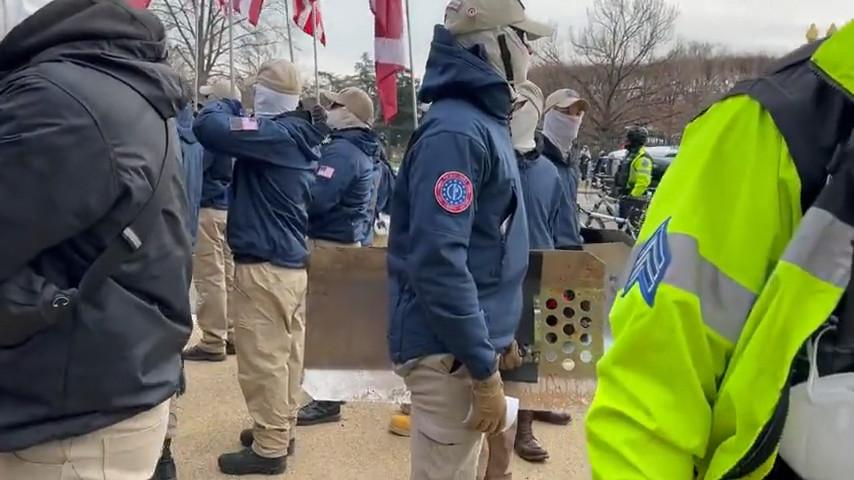
\includegraphics[width=\textwidth,height=0.75\textheight]{img/patriot_lol.jpg}}{img/patriot_lol.mp4}

  \footnotesize
  \url{https://twitter.com/socialistdogmom/status/1484598113096634379}
\end{frame}

\begin{frame}
  \frametitle{Patriot Front (2022)}
  \framesubtitle{\url{https://ddosecrets.com/wiki/Patriot_Front}}

  \centering
  \movie[width=\textwidth,height=0.75\textheight]{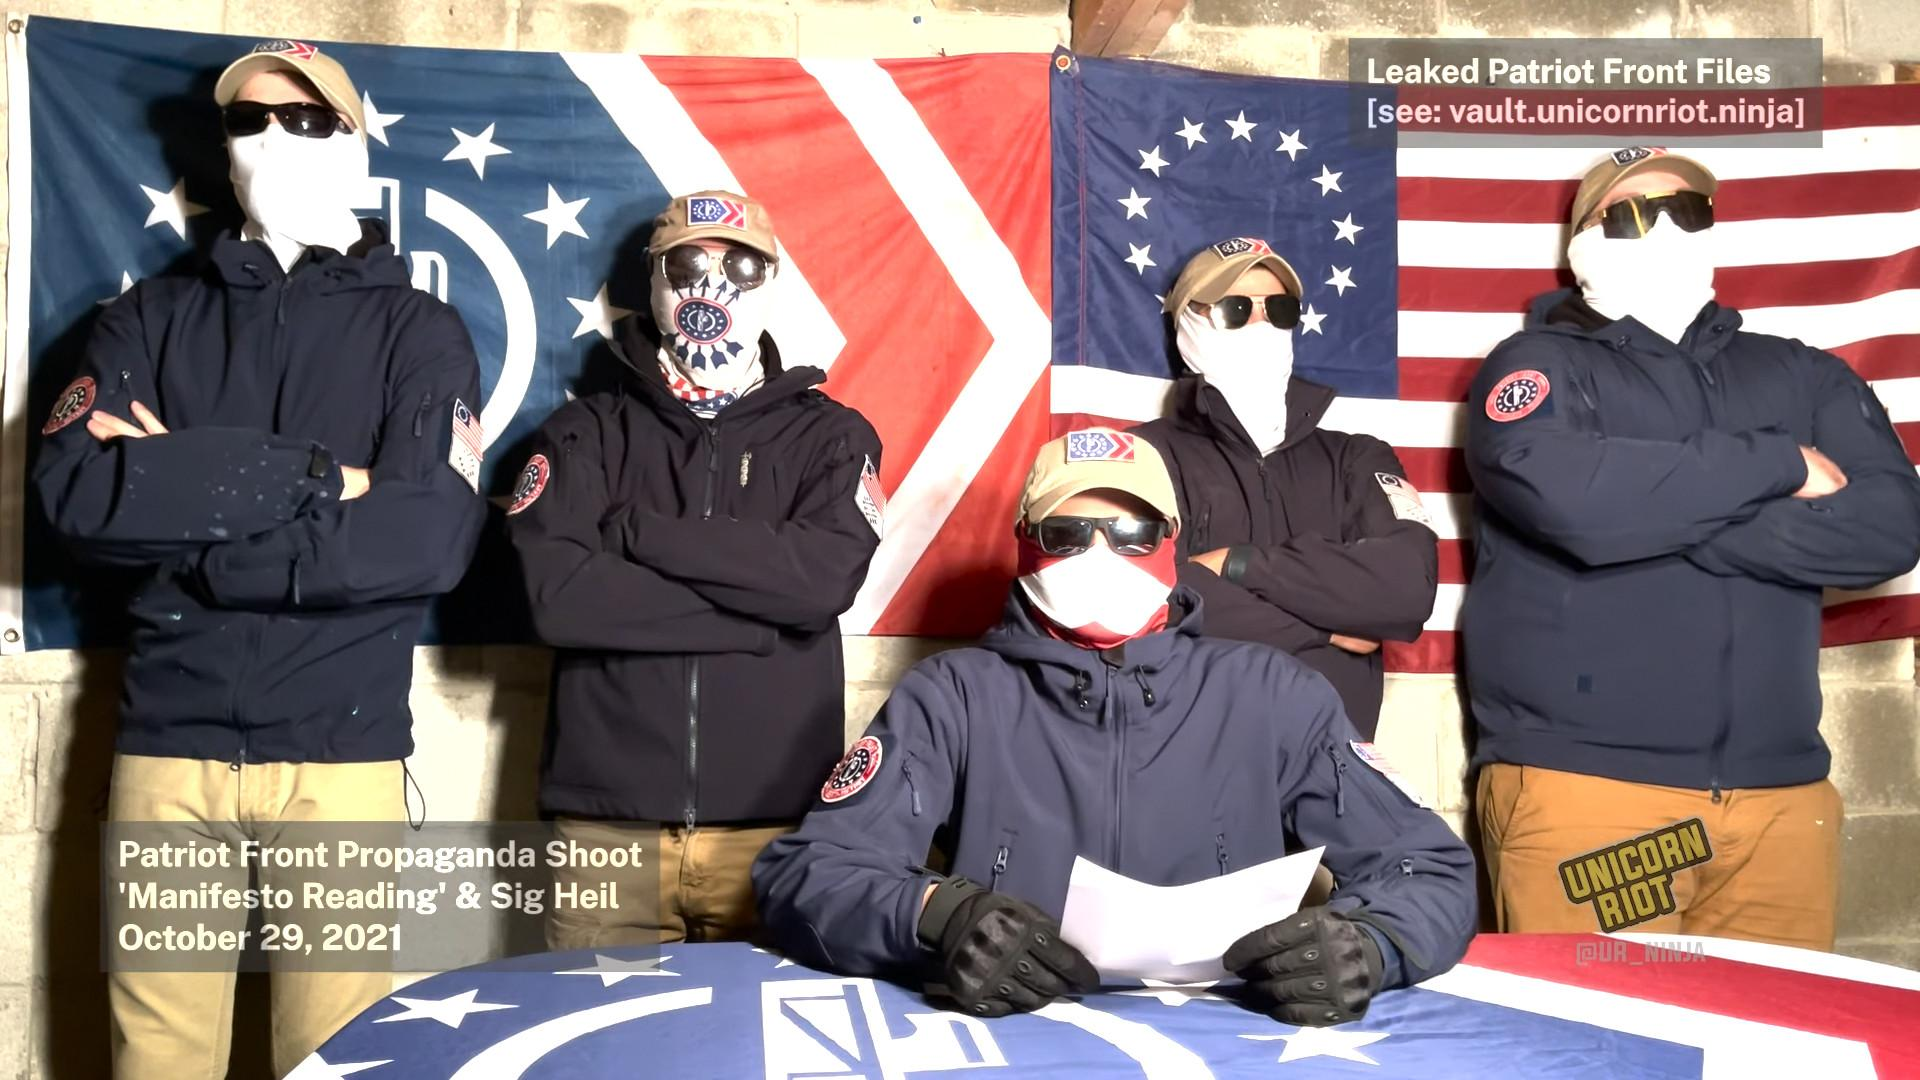
\includegraphics[width=\textwidth,height=0.75\textheight]{img/patriot_lol2.jpg}}{img/patriot_lol2.mp4}

  \footnotesize
  \url{https://www.youtube.com/watch?v=nywZLu0M_VY}
\end{frame}

%%% hillary video
\begin{frame}
  \frametitle{War in Ukraine}

  \centering
  \movie[width=\textwidth,height=0.75\textheight]{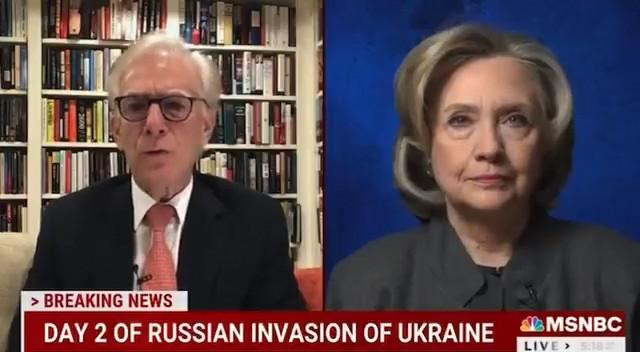
\includegraphics[width=\textwidth,height=0.75\textheight]{img/hillary_anonymous_do_something.jpg}}{img/hillary_anonymous_do_something.mp4}
\end{frame}

%% Roskomnadzor (2022)
\begin{frame}
  \frametitle{Roskomnadzor (2022)}
  \framesubtitle{\url{https://ddosecrets.com/wiki/Roskomnadzor}}

  \begin{itemize}[<+->]
    \item At the beginning of the war, factual information
      about the war was increasing getting suppressed from the Russian
      internet.
    \item In addition to the on-the-street repression of anti-war protesters,
      expressing opposition to the war on social media was being
      met with real life consequences.
    \item The agency in charge of monitoring, controlling and censoring
      Russian mass media, as well as the Internet is Roskomnadzor.
    \item There were rumours going around that Roskomnadzor was going to cut
      off Russia completely from the outside Internet, instituting a
      Chinese-style great firewall.
  \end{itemize}
\end{frame}

\begin{frame}
  \frametitle{Roskomnadzor (2022)}
  \framesubtitle{\url{https://ddosecrets.com/wiki/Roskomnadzor}}

  \begin{itemize}[<+->]
    \item The Roskomnadzor office in Bashkorstan got hacked by Anonymous and
      data was provided to Distributed Denial of Secrets.
    \item Investigated by independent Russian media outlet Meduza and the New
      York Times.
    \item Revealed that Russia's federal government has been monitoring the
      internet for peace activism since 2020.
  \end{itemize}

  \vfill
  \centering \pause

  \footnotesize
  \url{https://meduza.io/en/feature/2022/04/13/the-hunt-for-antimilitarism}\\

  \vspace{1mm}

  \url{https://www.nytimes.com/interactive/2022/09/22/technology/russia-putin-surveillance-spying.html}

\end{frame}

%% OpRussia (2022)
\begin{frame}
  \frametitle{OpRussia (2022)}
  \framesubtitle{\url{https://ddosecrets.com/wiki/Category:Russia}}

  \begin{itemize}[<+->]
    \item The brutality of what was happening in Ukraine, seeing innocent
      people getting killed and displaced was a call to action for many
      hacktivist groups, including Anonymous, the Belarusian Cyber-Partisans,
      Network Batallion 65, the Ukrainian IT army and many more.
    \item Many saw it as a free-for-all and a chance to hack without the risk
      of legal consequences, if they never planned to visit Russia anyway.
    \item Even some white-hats decided to get involved, seeing it as an
      opportunity to finally \emph{"HackBack!"} against the evil Russian
      hackers that they had to deal with in their daily work.
  \end{itemize}

\end{frame}

\begin{frame}
  \frametitle{OpRussia (2022)}
  \framesubtitle{\url{https://ddosecrets.com/wiki/Category:Russia}}

  \begin{itemize}[<+->]
    \item There were too many actions that took place during this time to go
      over them individually.
    \item After a few months most people seem to have got bored, but there
      are still some new hacks and leaks popping up out of Russia from time
      to time, but not at the same insane pace that we saw in the middle of
      2022.
  \end{itemize}

\end{frame}

\begin{frame}[t]
  \frametitle{OpRussia (2022)}
  \framesubtitle{\url{https://ddosecrets.com/wiki/Category:Russia}}

  \begin{columns}[T]
    \footnotesize
    \column{.45\textwidth}
    \begin{itemize}
      \item \href{https://ddosecrets.com/wiki/Accent_Capital}{\textcolor{blue}{Accent Capital}}
      \item \href{https://ddosecrets.com/wiki/Achinsk_City_Government}{\textcolor{blue}{Achinsk City Government}}
      \item \href{https://ddosecrets.com/wiki/Aerogas}{\textcolor{blue}{Aerogas}}
      \item \href{https://ddosecrets.com/wiki/ALET}{\textcolor{blue}{ALET}}
      \item \href{https://ddosecrets.com/wiki/Blagoveshchensk_City_Administration}{\textcolor{blue}{Blagoveshchensk City Administration}}
      \item \href{https://ddosecrets.com/wiki/Capital_Legal_Services}{\textcolor{blue}{Capital Legal Services}}
      \item \href{https://ddosecrets.com/wiki/Central_Bank_of_Russia}{\textcolor{blue}{Central Bank of Russia}}
      \item \href{https://ddosecrets.com/wiki/Continent_Express}{\textcolor{blue}{Continent Express}}
      \item \href{https://ddosecrets.com/wiki/Convex}{\textcolor{blue}{Convex}}
      \item \href{https://ddosecrets.com/wiki/CorpMSP}{\textcolor{blue}{CorpMSP}}
    \end{itemize}
    \column{.45\textwidth}
    \begin{itemize}
      \item \href{https://ddosecrets.com/wiki/Dept_of_Education_of_the_Strezhevoy_City_District_Administration}{\textcolor{blue}{Dept of Education of the Strezhevoy City District Administration}}
      \item \href{https://ddosecrets.com/wiki/Dept._for_Church_Charity_and_Social_Service_of_the_Russian_Orthodox_Church}{\textcolor{blue}{Dept. for Church Charity and Social Service of the Russian Orthodox Church}}
      \item \href{https://ddosecrets.com/wiki/Elektrocentromontazh}{\textcolor{blue}{Elektrocentromontazh}}
      \item \href{https://ddosecrets.com/wiki/Elvees}{\textcolor{blue}{Elvees}}
      \item \href{https://ddosecrets.com/wiki/Embassy_of_Ecuador,_Moscow}{\textcolor{blue}{Embassy of Ecuador, Moscow}}
      \item \href{https://ddosecrets.com/wiki/Enerpred}{\textcolor{blue}{Enerpred}}
      \item \href{https://ddosecrets.com/wiki/Forest}{\textcolor{blue}{Forest}}
      \item \href{https://ddosecrets.com/wiki/FSB_employee_leak}{\textcolor{blue}{FSB employee leak}}
      \item \href{https://ddosecrets.com/wiki/Gazprom_Linde_Engineering}{\textcolor{blue}{Gazprom Linde Engineering}}
      \item \href{https://ddosecrets.com/wiki/Gazregion}{\textcolor{blue}{Gazregion}}
    \end{itemize}
  \end{columns}
\end{frame}

\begin{frame}[t]
  \frametitle{OpRussia (2022)}
  \framesubtitle{\url{https://ddosecrets.com/wiki/Category:Russia}}

  \begin{columns}[T]
    \footnotesize
    \column{.45\textwidth}
    \begin{itemize}
      \item \href{https://ddosecrets.com/wiki/GUOV_I_GS_-_General_Dept._of_Troops_and_Civil_Construction}{\textcolor{blue}{GUOV I GS - General Dept. of Troops and Civil Construction}}
      \item \href{https://ddosecrets.com/wiki/LLC_Capital}{\textcolor{blue}{LLC Capital}}
      \item \href{https://ddosecrets.com/wiki/Marathon_Group}{\textcolor{blue}{Marathon Group}}
      \item \href{https://ddosecrets.com/wiki/MashOil}{\textcolor{blue}{MashOil}}
      \item \href{https://ddosecrets.com/wiki/McLanahan_Russia}{\textcolor{blue}{McLanahan Russia}}
      \item \href{https://ddosecrets.com/wiki/Metprom_Group}{\textcolor{blue}{Metprom Group}}
      \item \href{https://ddosecrets.com/wiki/Ministry_of_Culture_of_the_Russian_Federation}{\textcolor{blue}{Ministry of Culture of the Russian Federation}}
      \item \href{https://ddosecrets.com/wiki/Mosekspertiza}{\textcolor{blue}{Mosekspertiza}}
      \item \href{https://ddosecrets.com/wiki/Neocom_Geoservice}{\textcolor{blue}{Neocom Geoservice}}
    \end{itemize}
    \column{.45\textwidth}
    \begin{itemize}
      \item \href{https://ddosecrets.com/wiki/NPO_VS}{\textcolor{blue}{NPO VS}}
      \item \href{https://ddosecrets.com/wiki/Petrofort}{\textcolor{blue}{Petrofort}}
      \item \href{https://ddosecrets.com/wiki/Polar_Branch_of_the_Russian_Federal_Research_Institute_of_Fisheries_and_Oceanography}{\textcolor{blue}{Polar Branch of the Russian Federal Research Institute of Fisheries and Oceanography}}
      \item \href{https://ddosecrets.com/wiki/Port_and_Railway_Projects_Service_of_JSC_UMMC}{\textcolor{blue}{Port and Railway Projects Service of JSC UMMC}}
      \item \href{https://ddosecrets.com/wiki/PSCB}{\textcolor{blue}{PSCB}}
      \item \href{https://ddosecrets.com/wiki/Public_Chamber_of_the_Krasnoyarsk}{\textcolor{blue}{Public Chamber of the Krasnoyarsk}}
      \item \href{https://ddosecrets.com/wiki/Rosatom}{\textcolor{blue}{Rosatom}}
      \item \href{https://ddosecrets.com/wiki/ROSOBORONEXPORT}{\textcolor{blue}{ROSOBORONEXPORT}}
    \end{itemize}
  \end{columns}
\end{frame}

\begin{frame}[t]
  \frametitle{OpRussia (2022)}
  \framesubtitle{\url{https://ddosecrets.com/wiki/Category:Russia}}

  \begin{columns}[T]
    \footnotesize
    \column{.45\textwidth}
    \begin{itemize}
      \item \href{https://ddosecrets.com/wiki/RostProekt}{\textcolor{blue}{RostProekt}}
      \item \href{https://ddosecrets.com/wiki/Russian_Interior_Ministry}{\textcolor{blue}{Russian Interior Ministry}}
      \item \href{https://ddosecrets.com/wiki/Russian_soldier_leak}{\textcolor{blue}{Russian soldier leak}}
      \item \href{https://ddosecrets.com/wiki/RussianCensorFiles}{\textcolor{blue}{RussianCensorFiles}}
      \item \href{https://ddosecrets.com/wiki/Sawatzky}{\textcolor{blue}{Sawatzky}}
      \item \href{https://ddosecrets.com/wiki/SOCAR_Energoresource}{\textcolor{blue}{SOCAR Energoresource}}
      \item \href{https://ddosecrets.com/wiki/Technoserv}{\textcolor{blue}{Technoserv}}
    \end{itemize}
    \column{.45\textwidth}
    \begin{itemize}
      \item \href{https://ddosecrets.com/wiki/Technotec}{\textcolor{blue}{Technotec}}
      \item \href{https://ddosecrets.com/wiki/Tendertech}{\textcolor{blue}{Tendertech}}
      \item \href{https://ddosecrets.com/wiki/Thozis_Corp}{\textcolor{blue}{Thozis Corp}}
      \item \href{https://ddosecrets.com/wiki/Transneft}{\textcolor{blue}{Transneft}}
      \item \href{https://ddosecrets.com/wiki/VGTRK}{\textcolor{blue}{VGTRK}}
      \item \href{https://ddosecrets.com/wiki/Vyberi_Radio}{\textcolor{blue}{Vyberi Radio}}
      \item \href{https://ddosecrets.com/wiki/Worldwide_Invest}{\textcolor{blue}{Worldwide Invest}}
    \end{itemize}
  \end{columns}
\end{frame}

%% Nauru Police Force (2022)
\begin{frame}
  \frametitle{Nauru Police Force (2022)}
  \framesubtitle{\url{https://ddosecrets.com/wiki/Nauru_Police_Force}}

  \begin{itemize}[<+->]
    \item Just before the Australian election in 2022, a group of
      hacktivists calling themselves "All (Cyber-)Cops Are Bastards!" released
      a leak of 285,635 emails from Nauru Police Force.
    \item Nauru is a small island nation, most of it made uninhabitable by
      phosphate mining, where Australia sends asylum-seekers and refugees
      arriving on boats to live in horrible conditions.
    \item The emails confirmed the abuses endured by the refugees, as well as
      that those with connections to the media, lawyers or family in Australia
      were closely watched by a private intelligence contractor - something
      the Australian government has previously denied.
  \end{itemize}

  \vfill \centering \footnotesize \pause
  \url{https://www.theguardian.com/australia-news/2022/aug/06/coalition-used-private-contractor-to-collect-intelligence-on-nauru-asylum-seekers}

\end{frame}

\begin{frame}
  \frametitle{Nauru Police Force (2022)}
  \framesubtitle{\url{https://ddosecrets.com/wiki/Nauru_Police_Force}}

  The hacktivists included a statement with the leak asking the newly elected
  Australian government to commit to closing the mandatory immigration
  detention center on the island of Nauru.

  \centering \footnotesize

  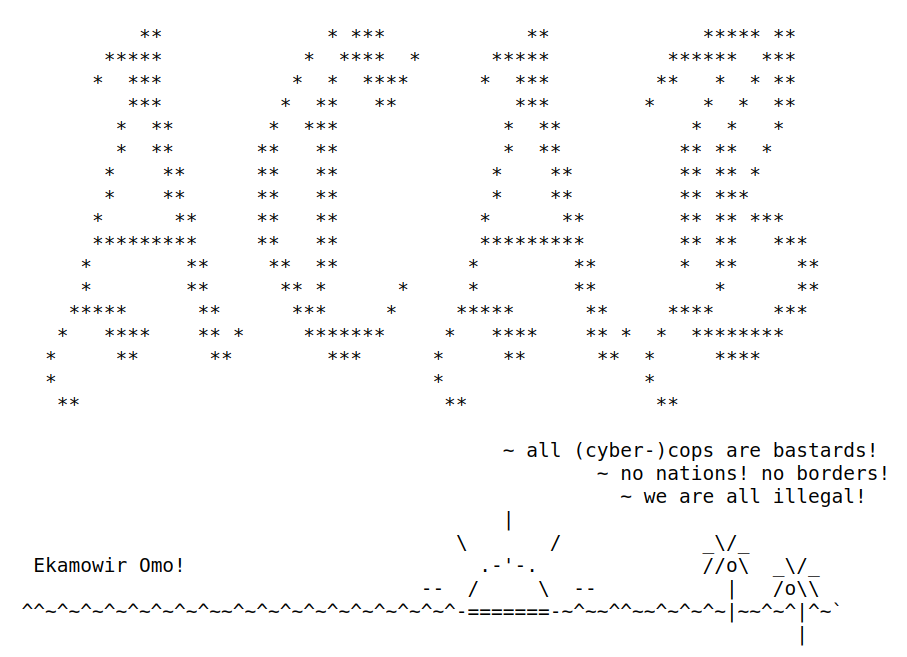
\includegraphics[width=\textwidth,height=0.5\textheight,keepaspectratio]{img/nauru_txt.png}

  \vfill

  \url{https://enlacehacktivista.org/nauru.txt}

\end{frame}

%% Pronico (2022)
\begin{frame}
  \frametitle{Guacamaya}

  \begin{itemize}[<+->]
    \item Also in 2022, what I find the most fascinating
      hacktivist group of all time, made an appearance.
    \item Guacamaya (Spanish name for Macaw parrot) is a collective of
      environmentalist hacktivists focused on hacks and leaks from the
      extractivist industry, law enforcement agencies and militaries in Abya
      Yala (native name for Central part of the American continent)
    \item Each of their hacks is accompanies by political statements (in
      Spanish,) poems, artwork and instructional videos in the same
      \emph{HackBack!} style pioneered by Phineas Fisher.
  \end{itemize}

  \vfill
  \footnotesize \centering \pause
  \url{https://www.vice.com/en/article/5d39j3/meet-the-environmental-hacktivists-trying-to-sabotage-mining-companies}

\end{frame}

\begin{frame}[c]
  \frametitle{Guacamaya}

  \centering
  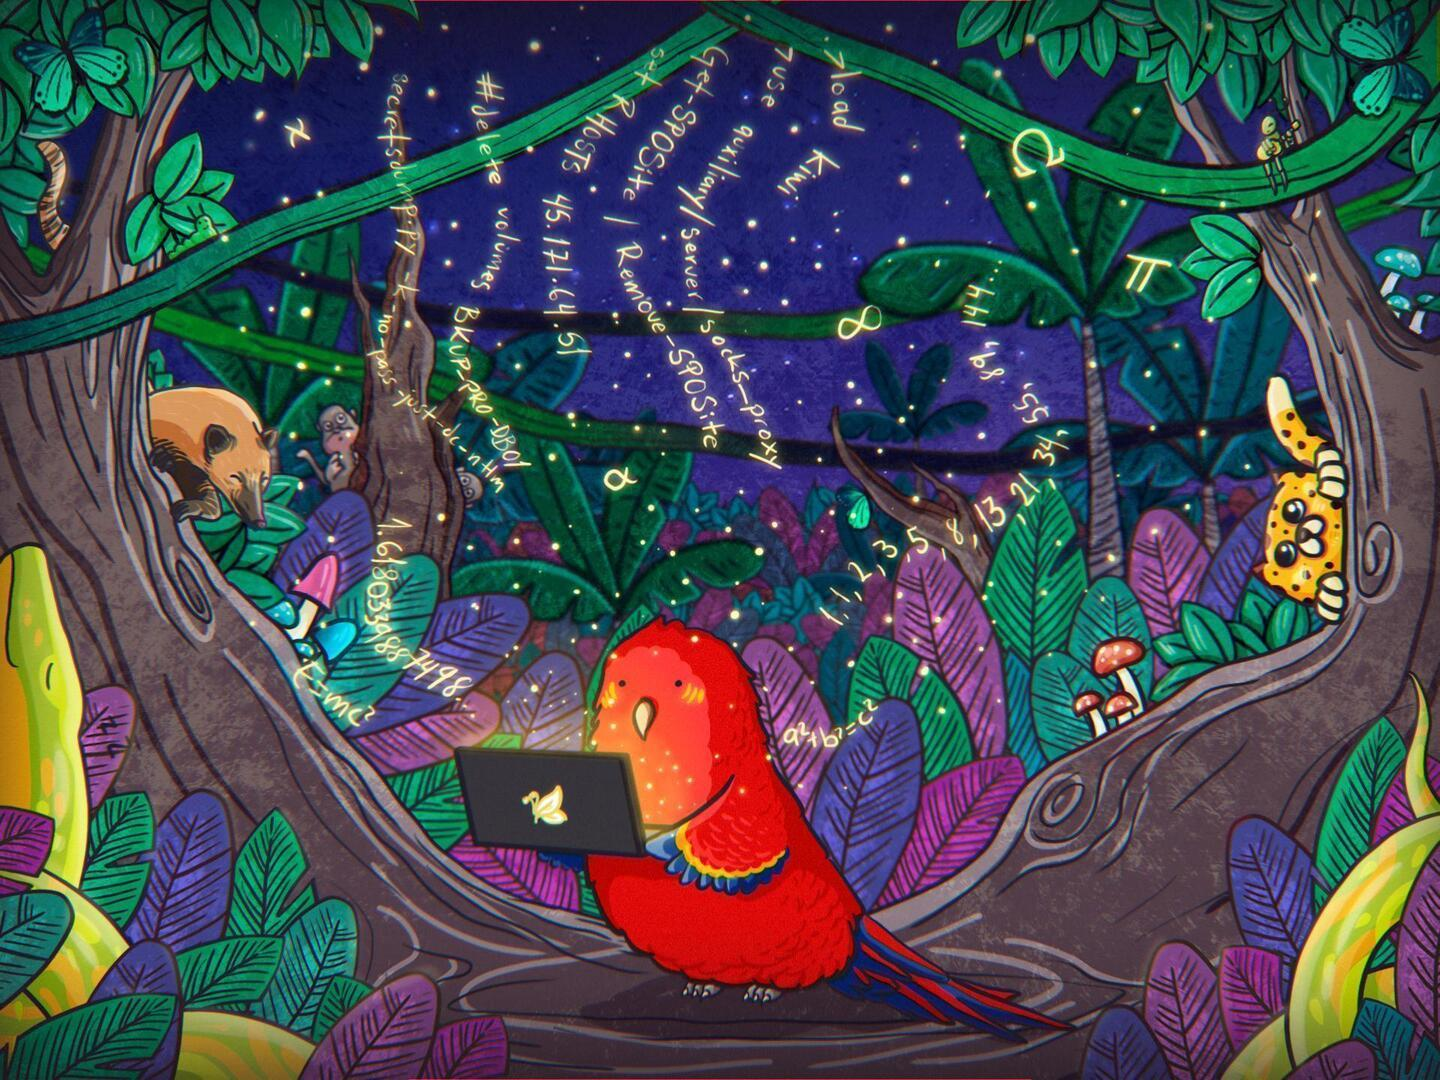
\includegraphics[width=\textwidth,height=0.7\textheight,keepaspectratio]{img/guacamaya.jpg}

  \footnotesize
  \emph{Artwork of Guacamaya, released alongside their first hack, of mining
  company Pronico}

\end{frame}

\begin{frame}
  \frametitle{Guacamaya}
  \framesubtitle{Mining Secrets (2022)}

  \begin{itemize}[<+->]
    \item Guacamaya's first hack was that of Pronico, a Swiss/Russian company
      that operates the Fenix mine in Guantamala.
    \item The mine had a long history of human rights abuses, environmental
      damage and resistance by the local communities.
    \item \url{https://forbiddenstories.org/case/mining-secrets/}
    \item \url{https://ddosecrets.com/wiki/Mining_Secrets}
  \end{itemize}
\end{frame}

\begin{frame}
  \frametitle{Guacamaya}
  \framesubtitle{Mining Secrets (2022)}

  \footnotesize
  The leak was accompanied by a video inspired by Phineas Fisher's
  \emph{HackBack!} series, titled \emph{HackBack!: A DIY Guide to Digital
  Monkeywrenching} - a full screen recording of the hack as it happened.

  \vfill \centering
  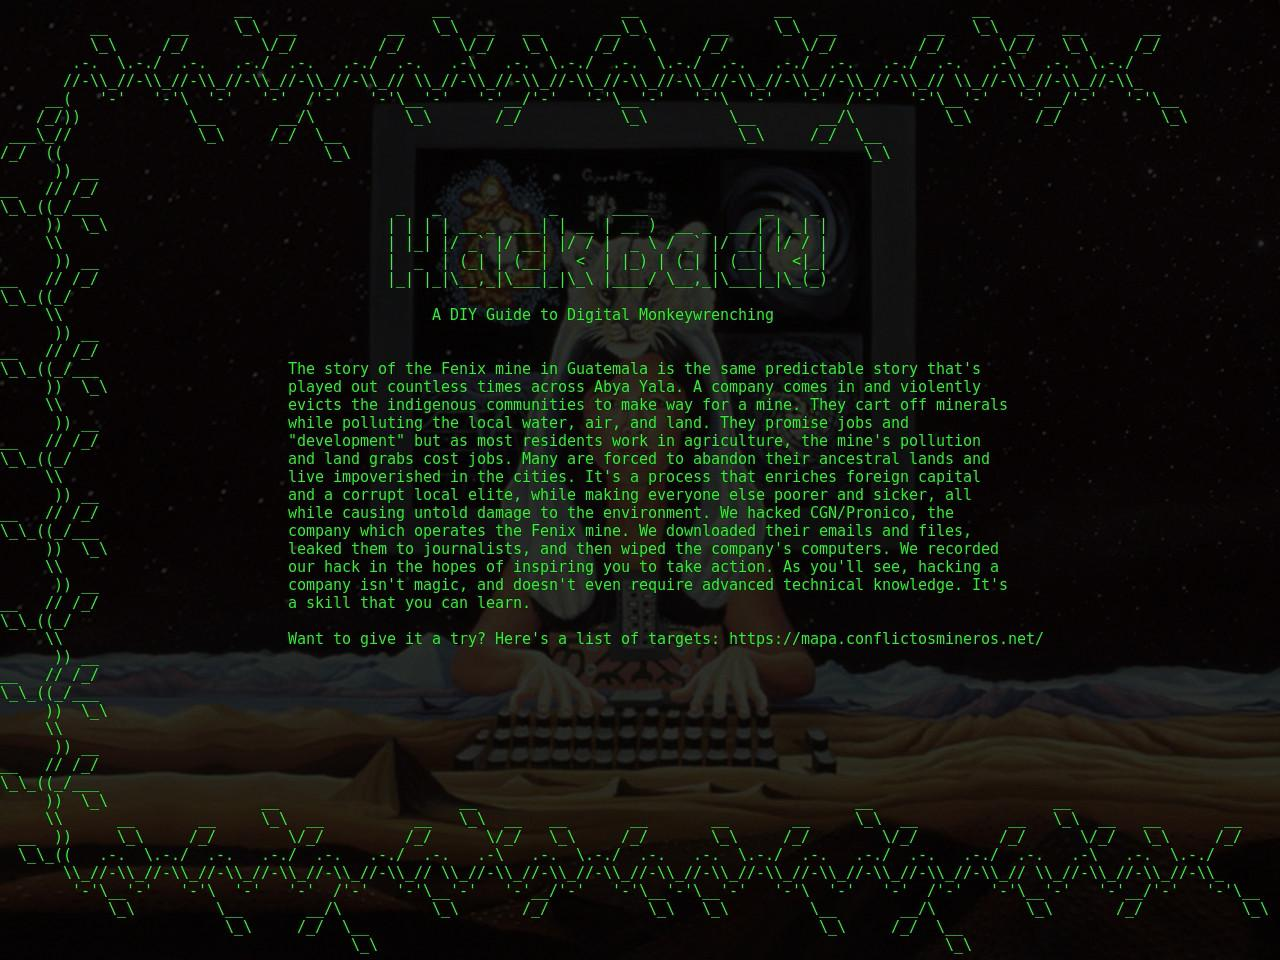
\includegraphics[width=\textwidth,height=0.6\textheight,keepaspectratio]{img/hackback_guacamaya.jpg}

  \url{https://kolektiva.media/w/twJjCTkvumnugRy61BjD3T}
\end{frame}

\begin{frame}[c]
  \frametitle{Guacamaya}

  \begin{quote}
    \textbf{How would you describe the role of a hacker like you in our
    society?}

    \vspace{3mm} \pause

    The role of a hacker is to take part in the different forms of resistance
    in any territory where there is dignified rage and a joyful desire for
    radical revolution.
  \end{quote}

  \vfill \scriptsize \centering
  \url{https://forbiddenstories.org/the-struggle-of-one-territory-must-be-the-struggle-of-all/}

\end{frame}
%% Extractivist Leaks (2022)
\begin{frame}
  \frametitle{Guacamaya}
  \framesubtitle{Extractivist Leaks (2022)}

  Emails from Ecuador's state mining company; Guatemala's ministry of natural
  resources; Colombia's hydrocarbons agency; and from oil and mining companies
  in Brazil, Venezuela, Chile and Colombia.

  \vfill \footnotesize \centering
  \url{https://ddosecrets.substack.com/p/extractivist-leaks-colombia-ecuador-chile-brazil}\\
  \vspace{1mm}
  \url{https://ddosecrets.com/wiki/Category:Extractivist_Leaks}

\end{frame}
%% Fuerzas Represivas (2022)
\begin{frame}
  \frametitle{Guacamaya}
  \framesubtitle{Fuerzas Represivas (2022)}

  \begin{itemize}[<+->]
    \item
      \href{https://ddosecrets.com/wiki/Fuerza_Armada_de_El_Salvador}{\textcolor{blue}{Armed Forces of El Salvador}}
    \item
      \href{https://ddosecrets.com/wiki/Comando_General_de_las_Fuerzas_Militares_de_Colombia}{\textcolor{blue}{General Command of the Military Forces of Colombia}}
    \item
      \href{https://ddosecrets.com/wiki/Estado_Mayor_Conjunto_de_las_Fuerza_Armadas_de_Chile}{\textcolor{blue}{Joint Chiefs of Staff of the Chilean Armed Forces}}
    \item
      \href{https://ddosecrets.com/wiki/Comando_Conjunto_de_las_Fuerzas_Armadas}{\textcolor{blue}{Joint Command of the Armed Forces of Peru}}
    \item
      \href{https://ddosecrets.com/wiki/Ej\%C3\%A9rcito_del_Per\%C3\%BA}{\textcolor{blue}{Peruvian Army}}
    \item
      \href{https://ddosecrets.com/wiki/Polic\%C3\%ADa_Nacional_Civil_de_El_Salvador}{\textcolor{blue}{National Civil Police of El Salvador}}
  \end{itemize}
\end{frame}

\begin{frame}[c]
  \frametitle{Guacamaya}
  \framesubtitle{Secretaría de la Defensa Nacional México (SEDENA) (2022)}

  Six terabytes of emails from Mexico's SEDENA, showing evidence of corruption
  in the military, plus their surveillance of politicians, diplomats, artists,
  activists and journalists.

  \vspace{5mm}

  Hundreds of news stories based on this leak alone:

  \vspace{5mm}

  \centering
  \scriptsize
  \href{https://ddosecrets.com/wiki/Secretar\%C3\%ADa_de_la_Defensa_Nacional_de_M\%C3\%A9xico\#Research}{\texttt{https://ddosecrets.com/wiki/Secretaría\_de\_la\_Defensa\_Nacional\_de\_México\#Research}}

\end{frame}

%% Supreme court leak (2022)
\begin{frame}
  \frametitle{Supreme Court Leak (2022)}

  \begin{itemize}[<+->]
    \item On May 2, 2022, Politico released a leaked draft of an opinion
      that would overturn Roe v. Wade, from an insider source in the Supreme
      Court of the United States.
    \item Effectively ending guaranteed right to abortion in the United
      States, leaving it up to state law.
    \item Caused huge backlash and protests, regardless the majority opinion
      was largely the same as the leaked draft.
    \item Approximetely 90 people would have had access to the document.
    \item So far, despite an investigation, the leaker was not caught.
  \end{itemize}

\end{frame}

%% Liberty Counsel (2022)
\begin{frame}
  \frametitle{Liberty Counsel (2022)}
  \framesubtitle{\url{https://ddosecrets.com/wiki/Liberty_Counsel}}

  The hackers also did their part.

  \footnotesize \pause \par
  \begin{quote}
    Liberty Counsel helped overturn Roe v. Wade, and claim to have prayed with
    Supreme Court justices. This release also includes more than 100 internal
    databases from mostly Christian missionary groups that use the same
    software for customer relationship management (CRM), called WMTEK.
    WMTEK develops software exclusively for non-profits that are supposedly
    Christian.

    \par \pause

    This collection includes about 450GB of databases once uncompressed,
    as well a git repositories and files found in the webroots of web servers.
    The data spans from 2015 to 2022 and includes PII for donors and
    supporters of these groups, as well as details about financial
    transactions. All together, these databases track hundreds of millions
    of dollars in donations to Christian groups.

    \par \pause

    The Liberty Counsel database is 25GB uncompressed, and includes
    262,000 people, 44,000 who are donors.

  \end{quote}

\end{frame}

%% Ariantel (2022)
\begin{frame}
  \frametitle{ArianTel (2022)}
  \framesubtitle{\url{https://ddosecrets.com/wiki/ArianTel}}

  \begin{itemize}[<+->]
    \item Mid-September a series of furious protests kicked off in Iran after
      a young woman named Mahsa Jina Amini was killed while in the custody of
      the country's morality police.
    \item The government's crackdown took a variety of shapes, including
      brute force and cutting off the country's access to the Internet.
    \item In support of protests, hackers hacked and leaked confidential
      emails from Iranian telecom provider, ArianTel.
  \end{itemize}
\end{frame}

\begin{frame}
  \frametitle{ArianTel (2022)}
  \framesubtitle{\url{https://ddosecrets.com/wiki/ArianTel}}

  \begin{itemize}[<+->]
    \item Revealed a secret government programme called SIAM enabling tracking
      of protesters, hijacking calls, SMS messages and cutting off network
      access to specific subscribers or selected areas.
    \item Every telecom provider is required to implement a version of the
      system and give access to Iran's Communications Regulatory Authority.
    \item The leak exposed technical specifications and manuals for the
      system, as well as western and Russian telecommunications equipment
      makers who helped implement it, via shell companies in UK and Portugal
      representing ArianTel, possibly violating economic sanctions
      against Iran.
    \item In Iran, every SIM card and IMEI has to be registered with the
      government to the user's identity. This includes roaming visitors to the
      country, who have 30 days to register their phone before service gets
      cut off.
  \end{itemize}
\end{frame}

\begin{frame}[c]
  \frametitle{ArianTel (2022)}
  \framesubtitle{\url{https://theintercept.com/2022/10/28/iran-protests-phone-surveillance/}}

  \footnotesize \centering

  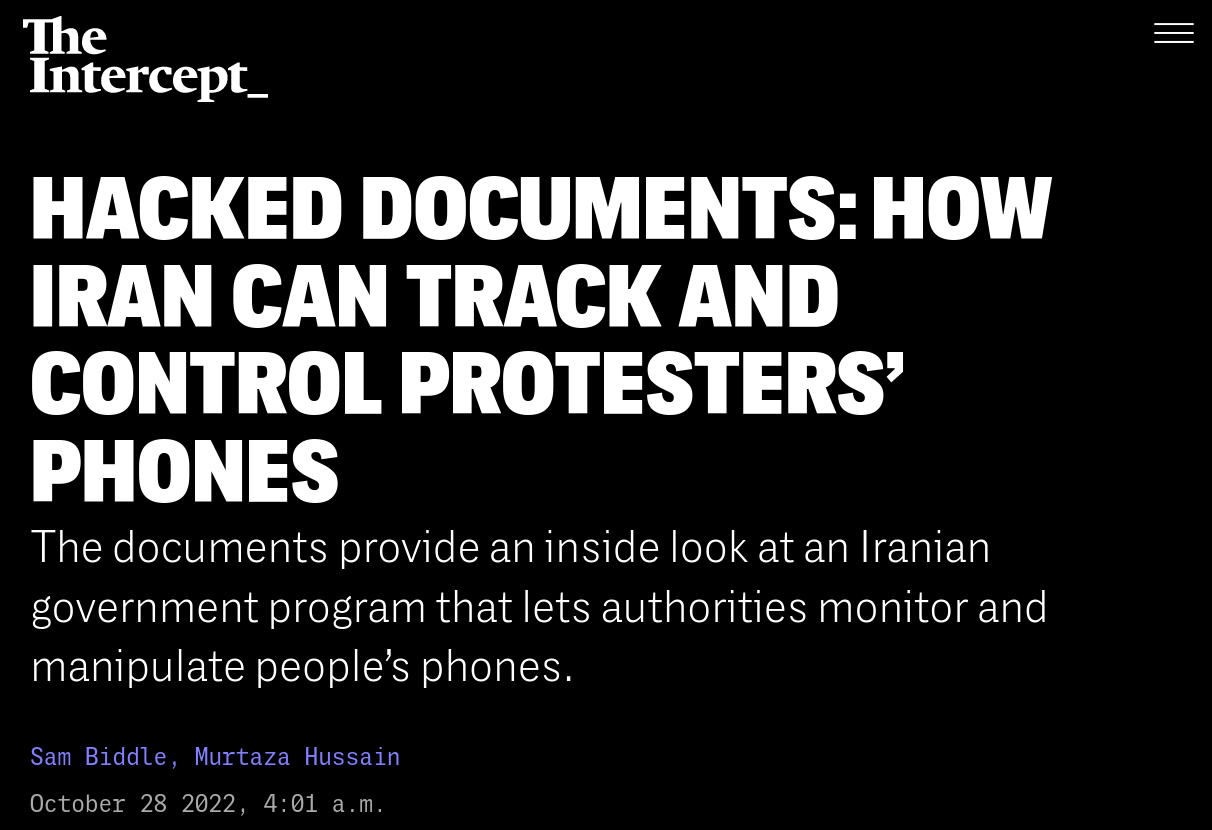
\includegraphics[width=\textwidth,height=0.6\textheight,keepaspectratio]{img/ariantel1.png}

  \vfill
  \emph{The Intercept - Hacked Documents: How Iran Can Track and Control
  Protesters' Phones}

\end{frame}

\begin{frame}[c]
  \frametitle{ArianTel (2022)}
  \framesubtitle{\url{https://citizenlab.ca/2023/01/uncovering-irans-mobile-legal-intercept-system/}}

  \footnotesize \centering

  \includegraphics[width=\textwidth,height=0.6\textheight,keepaspectratio]{img/ariantel2.png}

  \vfill
  \emph{The Citizen Lab - You Move, They Follow - Uncovering Iran's Mobile
  Legal Intercept System}

\end{frame}

%% Myanmar Internal Revenue Department (2023)
\begin{frame}[c]

  \LARGE
  \centering 2023

\end{frame}

\begin{frame}[c]
  \frametitle{Myanmar Internal Revenue Department (2023)}
  \framesubtitle{\url{https://ddosecrets.com/wiki/Myanmar_Internal_Revenue_Department}}

  \begin{itemize}[<+->]
    \item Leak of every tax filing from the Myanmar's Internal Revenue
      Department, state agency that has been illegally controlled by the
      Myanmar Military since the coup in February 2021.
    \item Details of large tax payments that have flowed into the junta's
      coffers.
    \item Used by ICIJ in their \emph{Deforestation Inc.} investigation,
      exposing western companies that illegally import teak from Myanmar to
      produce yacht decks, often while having green sustainable forestry
      certifications.
  \end{itemize}

  \vfill \footnotesize \centering \pause
  \url{https://www.icij.org/investigations/deforestation-inc/auditors-green-labels-sustainability-environmental-harm/}
\end{frame}

%% nofly.csv (2023)
\begin{frame}
  \frametitle{nofly.csv (2023)}
  \framesubtitle{\url{https://maia.crimew.gay/posts/how-to-hack-an-airline/}}

  \footnotesize
  maia arson crimew reappears with a leak of the U.S. TSA No Fly and Selectee
  screening lists.

  \centering \vfill
  \includegraphics[width=\textwidth,height=0.6\textheight,keepaspectratio]{img/weed-cat-crimes.jpg}

  \emph{"holy shit, we actually have the nofly list. holy fucking bingle.
  what?! :3"}

\end{frame}

%% 2600 pages of trans hate (2023)
\begin{frame}
  \frametitle{2600 pages of trans hate (2023)}
  \framesubtitle{\url{https://maia.crimew.gay/posts/the-emails/}}

  \begin{itemize}[<+->]
    \item A collection of emails from 2019-2021 between dozens of anti-trans
      expert witnesses, US right-wing lawmakers and conservative legal groups.
    \item Initially provided to
      \href{https://www.motherjones.com/politics/2023/03/anti-trans-transgender-health-care-ban-legislation-bill-minors-children-lgbtq/}{\textcolor{blue}{Mother
      Jones}} by an insider source.
    \item Later given to maia for wider re-distribution.
    \item Part 2: \url{https://maia.crimew.gay/posts/the-emails-2/}
  \end{itemize}

\end{frame}

%% most data leaks don't end up in hands of journalists
\begin{frame}
  \frametitle{Most data leaks don't end up in hands of journalists}

  \centering \footnotesize

  \includegraphics[width=\textwidth,height=0.7\textheight,keepaspectratio]{img/biggest_data_breaches.png}

  \emph{Graphic: World's Biggest Data Breaches}
\end{frame}

%% source protection:
\begin{frame}[c]

  \centering \LARGE
  source protection

\end{frame}
%% two types of sources:
\begin{frame}
  \frametitle{Types of sources}
  \framesubtitle{The Insider Leaker}

  \begin{itemize}[<+->]
    \item A source within an organization wishing to get information out from
      the inside.
    \item A whistleblower.
    \item Not necessary technical, may not know the necessary steps to take to
      protect their identity and communicate securely.
  \end{itemize}

\end{frame}

\begin{frame}
  \frametitle{Types of sources}
  \framesubtitle{The Insider Leaker}

  \begin{itemize}[<+->]
    \item The main question to ask when protecting an insider source:
    \item How many people had access to the information or documents the
      source wishes to get out?
    \item The likelihood of getting caught is inversely proportional to the
      number of people who accessed the document.
    \item Leaking information few people could or had recently accessed - very
      likely to get caught.
    \item Leaking an email that was sent to all employees of the
      organization - a lot less likely to get caught.
  \end{itemize}

\end{frame}

\begin{frame}
  \frametitle{Types of sources}
  \framesubtitle{The Insider Leaker}

  \begin{itemize}[<+->]
    \item When Reality Winner leaked a classified NSA document showing
      Russians were interfering in the U.S. elections, a lot of people put
      blame on The Intercept.
    \item Published scan of original document with hidden dots encoding the
      printer's serial number.
    \item When colour laser printers came onto the market, this
      feature was mandated by the U.S. Government out of concern the printers'
      quality was good enough to produce counterfeit bills.
    \item It was certainly a mistake by The Intercept to publish a scan of the
      original document (they could have reproduced a copy with OCR.)
    \item The leaked document was only viewed by three people inside the NSA.
    \item There was enough evidence produced to narrow it down to three people
      before Reality ever put it in the envelope to send to The Intercept.
  \end{itemize}

\end{frame}

\begin{frame}
  \frametitle{Types of sources}
  \framesubtitle{The Insider Leaker}

  \begin{itemize}[<+->]
    \item Things have changed a lot in the last 10 years.
    \item Organizations are wary of insider threats and there are data loss
      prevention (DLP) and forensics software solutions marketed to prevent
      and investigate them.
    \item Employee surveillance is pervasive.
    \item The endpoint protection (anti-virus) software on your work computer
      is watching your every move.
    \item The days you could copy all company's files onto a microSD card
      and hide it inside a Rubik's cube are mostly gone, especially in large
      organizations with robust information security procedures.
  \end{itemize}

\end{frame}

\begin{frame}
  \frametitle{Types of sources}
  \framesubtitle{The Insider Leaker}

  \begin{itemize}[<+->]
    \item Secretive companies with lots of interest in leaks from
      journalists, like Apple and Tesla have employed other tricks to catch
      insider leakers.
    \item Secret messages encoded in extra whitespaces added to the document
      or email.
    \item Slight variations in wording for email sent to each suspected
      employee.
    \item Watermarking images and embedding metadata in the document.
    \item Always retype or use optical character recognition to recreate the
      original document.
    \item When in doubt, don't publish the source material.
  \end{itemize}

\end{frame}

\begin{frame}
  \frametitle{mat2}
  \framesubtitle{\url{https://0xacab.org/jvoisin/mat2}}

  \begin{itemize}[<+->]
    \item Tool for scrubbing metadata and other potentially identifiable
      infomation from images and documents.
    \item Removes GPS metadata, timestamp and camera model from photos and
      videos.
    \item Removes author information from Office documents and PDFs.
    \item Not fool proof.
    \item Would not work against things like the printer dots or the tricks
      used by Apple and Tesla.
  \end{itemize}

\end{frame}
%\end{frame}
%% hacker
\begin{frame}
  \frametitle{Types of sources}
  \framesubtitle{The Hacker}

  \begin{itemize}[<+->]
    \item Technical and likely already knows what steps to take to protect
      their identity online.
    \item Have a tendency to overestimate how much technology like Tor, VPNs
      and full disk encryption is going to protect them.
    \item The biggest threat to the hacker is their ego.
    \item A lot more likely to get caught bragging about their exploits to
      their friends than the FBI or NSA being able to break Tor.
  \end{itemize}
\end{frame}

\begin{frame}
  \frametitle{Types of sources}
  \framesubtitle{The Hacker}

  \centering
  \movie[width=\textwidth,height=0.75\textheight]{\includegraphics[width=\textwidth,height=0.75\textheight]{img/uber_hacker.jpg}}{img/uber_hacker.mp4}

  \footnotesize
  \href{https://youtu.be/aSSqLLeGdHI?t=239}{\textcolor{blue}{Hackers in Wonderland  (2000, Russel Barnes)}}

\end{frame}

\begin{frame}[c]
  \frametitle{Types of Sources}
  \framesubtitle{Are hackers whistleblowers?}

  \pause \large \centering
  \emph{truthtellers}
\end{frame}

%% communication with sources
\begin{frame}[c]

  \LARGE
  \centering
  communication with sources

\end{frame}

% signal
\begin{frame}
  \frametitle{Signal}
  \framesubtitle{\url{https://signal.org/}}

  \begin{itemize}[<+->]
    \item The most secure \emph{mainstream} instant messaging app available
      today.
    \item By \emph{mainstream} I mean it's something you could teach and
      convince your grandparents to use.
  \end{itemize}

\end{frame}

\begin{frame}
  \frametitle{Signal}
  \framesubtitle{\url{https://signal.org/}}

  \begin{itemize}[<+->]
    \item Uses phone numbers as identifiers.
    \item It does not need to be \emph{your actual phone number.}
    \item It is entirely possible to use Signal anonymously, it just takes a
      little creativity.
    \item Any phone number that can receive SMS or a phone call can be a
      Signal number.
    \item A VoIP number can be a Signal number. A Twilio number can be a
      Signal number. A public telephone booth can be a Signal number.
      A "receive SMS for free" website can be a Signal number.
    \item Just remember to turn on registration lock.
  \end{itemize}
\end{frame}

\begin{frame}
  \frametitle{Signal}
  \framesubtitle{\url{https://signal.org/}}

  \begin{itemize}[<+->]
    \item The main security property of Signal is not its strong encryption.
    \item Other popular messaging apps like WhatsApp also use the same Signal
      encryption protocol.
    \item It is that it has no facility for cloud chat backups.
    \item Your device has to be physically seized or compromised by malware to
      gain access to your messages.
    \item When subpoenaed, Signal can only provide law enforcement with date
      the account was created and last accessed. They publish every request
      for data and the response on their website.
    \item \url{https://signal.org/bigbrother/}
  \end{itemize}
\end{frame}

%% cwtch.im
\begin{frame}
  \frametitle{Cwtch}
  \framesubtitle{\url{https://cwtch.im/}}

  \begin{itemize}[<+->]
    \item Decentralized, metadata-resistant instant messenger, with encrypted
      messages exchanged peer-to-peer via Tor onion hidden services.
    \item Uses Tor v3 Onion hidden service public keys as identifiers.
    \item \texttt{4y2hxlxqzautabituedksnh2ulcgm2coqbure6wvfpg4gi2ci25ta5ad}
    \item The user experience encourages good habits like no logging and
      multiple ephemeral identities.
    \item Does not support asynchronous communication. Contacts have to be
      online at the same time.
    \item Still in early development. The mobile clients are buggy. Use the
      desktop client.
    \item Experimental support for file transfers.
    \item \url{https://openprivacy.ca/donate}
  \end{itemize}

\end{frame}

%% onionshare
\begin{frame}
  \frametitle{Onionshare}
  \framesubtitle{\url{https://onionshare.org/}}

  \begin{itemize}[<+->]
    \item OnionShare is an open source tool that lets you securely and
      anonymously share files, host websites, and chat with friends using
      the Tor network.
    \item Originally developed by Micah Lee, director of information security
      at The Intercept and member of the Tor Project. Now Freedom of the Press
      foundation.
    \item Easy to use graphical tool for sharing files securely over Tor,
      has a built-in chat function.
    \item Can be used to host a simple anonymous dropbox as a Tor hidden
      service. Does not have the same security properties as SecureDrop, but a
      lot easier to set up.
    \item Unsuitable for large file transfers. Interrupted transfers do not
      get resumed. Files get copied and compressed in memory, so file size
      is limited by RAM size.
  \end{itemize}

\end{frame}

%% pgp actually kinda sucks
\begin{frame}
  \frametitle{PGP/GnuPG email}

  \begin{itemize}[<+->]
    \item Not recommended.
    \item Difficult to use, only ever encrypts the content of the emails and
      not the metadata - who's communicating with whom.
    \item Obtuse user interface, a lot of opportunities to shoot yourself in
      the foot.
    \item Not only does it not protect who's communicating with whom, it
      confirms that they have something to hide.
    \item When a source is compromised, has a tendency of turning from
      \emph{Pretty Good Privacy} into \emph{Cryptographically Verifiable
      Evidence.}
    \item Stay away unless your source insists on it.
  \end{itemize}

\end{frame}

%% coy.im
\begin{frame}
  \frametitle{Jabber/XMPP}
  \framesubtitle{\url{https://coy.im/}}

  \begin{itemize}[<+->]
    \item No encryption by default, typically used with Off-the-Record (OTR)
      extension for end-to-end encryption.
    \item Has the same issue as PGP email, only the content of the messages
      is encrypted, your contact list is stored unencrypted on the server.
    \item The XMPP protocol is a lot more complicated than email,
      different clients support different sets of extensions,
      some problematic for privacy.
    \item For example, most clients will reveal your computer's timezone,
      which can compromise your physical location.
  \end{itemize}

\end{frame}

\begin{frame}
  \frametitle{Jabber/XMPP}
  \framesubtitle{\url{https://coy.im/}}

  \begin{itemize}[<+->]
    \item If your source insists on using it, the most secure client is
      probably Ola Bini's CoyIM.
    \item \url{https://coy.im/}
    \item Comes preconfigured with Tor, OTR and no logging by default.
      Supports only the basic XMPP features.
    \item Pidgin and Adium are a mess of 20-year-old unaudited spaghetti C
      code. Nobody should be using these for secure communications in 2023.
  \end{itemize}

\end{frame}

%% imessage, wire, threema, telegram, whatsapp, twitter dms really do suck
\begin{frame}
  \frametitle{Seriously, do not use these}

  \begin{itemize}[<+->]
    \item Burner feature phones - do not support end-to-end encrypted
      communications.
    \item iMessage - unencrypted cloud backups.
    \item Telegram - unencrypted by default, invented their own encryption
      protocol, cloud chat backups.
    \item Threema - invented their own encryption protocol from scratch, it's
      not good.
    \item Twitter DMs - unencrypted.
    \item WhatsApp - unencrypted cloud chat backups.
    \item Wire - logs your approximate geographical location.
  \end{itemize}

  \vfill \centering \footnotesize

  \url{https://www.documentcloud.org/documents/21114562-jan-2021-fbi-infographic-re-lawful-access-to-secure-messaging-apps-data}

\end{frame}

%% secure phones (plug grapheneos)
\begin{frame}
  \frametitle{Secure phones - GrapheneOS}
  \framesubtitle{\url{https://grapheneos.org/}}

  \begin{itemize}[<+->]
    \item The most secure phone you can get today is a Google Pixel running
      GrapheneOS.
    \item Fork of Android focused on privacy and security.
    \item Reduced attack surface and security hardening makes compromise
      by malware more difficult.
    \item Security model includes protecting the user's privacy from untrusted
      apps.
    \item You can even run Google Play Services without Google getting any
      personally identifiable information from the operating system!
  \end{itemize}
\end{frame}

\begin{frame}
  \frametitle{Secure phones - GrapheneOS}
  \framesubtitle{\url{https://grapheneos.org/}}

  \begin{itemize}[<+->]
    \item Network permission toggle and storage access scopes for apps.
    \item LTE only mode to prevent stingray downgrade attacks.
    \item Automatic reboot into full disk encryption lock down mode (before
      first unlock) when device left inactive.
    \item And more: \url{https://grapheneos.org/features}
  \end{itemize}

\end{frame}

\begin{frame}[c]

  \centering
  \url{https://ddosecrets.com/wiki/Tools_of_the_Trade}

\end{frame}

%% data sources
\begin{frame}[c]

  \LARGE
  \centering
  data sources

\end{frame}

%% ddosecrets.com
\begin{frame}
  \frametitle{Distributed Denial of Secrets}
  \framesubtitle{\url{https://ddosecrets.com/}}

  \centering
  \includegraphics[width=\textwidth,height=0.6\textheight,keepaspectratio]{img/ddosecrets_current.png}

  \vfill \centering \footnotesize
  \emph{Screenshot of the current Distributed Denial of Secrets home page}

\end{frame}

%% enlace hacktivista
\begin{frame}
  \frametitle{Enlace Hacktivista}
  \framesubtitle{\url{https://enlacehacktivista.org/}}

  \centering
  \includegraphics[width=\textwidth,height=0.6\textheight,keepaspectratio]{img/enlace_hacktivista.png}

  \vfill \footnotesize
  \emph{Screenshot of the current Enlace Hacktivista home page}

\end{frame}

\begin{frame}
  \frametitle{Enlace Hacktivista}
  \framesubtitle{\url{https://enlacehacktivista.org/}}

  \begin{itemize}[<+->]
    \item Launched in early 2022.
    \item More radical than Distributed Denial of Secrets, the editorial team
      is anonymous, publishes instructional hacking material and communiques
      from hackers, in addition to leaks.
    \item Most content gets mirrored by Distributed Denial of Secrets.
    \item Focused on preserving hacker history and sharing educational
      resources for hackers and those who want to learn.
  \end{itemize}

\end{frame}

%% torrents
\begin{frame}
  \frametitle{BitTorrent}
  \framesubtitle{How do I download data from a torrent?}

  \centering
  \LARGE
  \url{https://ddosecrets.com/wiki/Torrents}

\end{frame}

%% forbidden stories
\begin{frame}
  \frametitle{Forbidden Stories}
  \framesubtitle{\url{https://forbiddenstories.org/}}

  \begin{itemize}[<+->]
    \item Not a source of data.
    \item If you are investigating something and have been threatened or feel
      at risk, Forbidden Stories will protect your stories.
    \item Operate the SafeBox Network for threatened journalists to securily
      share their sensitive information.
    \item If something happens to you, Forbidden Stories will continue the
      investigation where you left off and publish your story.
  \end{itemize}

\end{frame}

%% dealing with data
\begin{frame}[c]

  \LARGE
  \centering
  dealing with data

\end{frame}

%% use a vm, tor, tails, qubes, or dedicated computer
\begin{frame}
  \frametitle{Safety First}
  \framesubtitle{Protect yourself}

  \begin{itemize}[<+->]
    \item Use a dedicated, disposable computer for working with the leaked
      data, preferably disconnected from the internet.
    \item Or a virtual machine.
    \item \href{https://www.torproject.org/}{\textcolor{blue}{Tor and Tor
      Browser}} to browse the Internet privately and bypass censorship.
    \item \href{https://tails.boum.org/}{\textcolor{blue}{Tails}} is a
      portable operating system that does not remember your activities
      and is pre-configured to use Tor by default. Can be used alongside your
      existing operating system booted from a USB stick.
    \item \href{https://www.qubes-os.org/}{\textcolor{blue}{Qubes OS}} is a
      security-oriented operating system that lets you compartmentalize your
      work into isolated virtual machines.
  \end{itemize}

\end{frame}

%% dangerzone
\begin{frame}[c]
  \frametitle{Dangerzone}
  \framesubtitle{\url{https://dangerzone.rocks/}}

  A tool to convert potentially dangerous PDFs, office documents, or images
  and convert them into safe PDFs.

\end{frame}

%% verifying documents
%% email (citizenlab)
\begin{frame}
  \frametitle{Verifying documents}

  \begin{itemize}[<+->]
    \item It's not always possible to verify the authenticity of a document
      just by looking at it.
    \item It may require traditional journalism work and cross-checking
      secondary sources.
    \item Generally, large sets of data are difficult to fake, who would
      have the time to create thousands of fake documents to leak to
      journalists?
    \item Metadata can be a giveaway that the data has been tampered with, for
      example, if there are discrepancies in file modification dates.
    \item The Citizen Lab made a tool specifically for verifying the integrity
      of leaked email datasets.
    \item \url{https://github.com/ninoseki/eml_analyzer}
  \end{itemize}

\end{frame}

%% helps to know your way around commandline, linux, a programming language
\begin{frame}
  \frametitle{Working with data}

  \begin{itemize}[<+->]
    \item When investigating leaked datasets, it helps to know your way around
      Linux and the command-line.
    \item I get a lot of mileage out of the venerable \texttt{grep},
      \texttt{sed} and \texttt{awk}.
    \item You will probably want to pick up at least one programming language,
      like Python and the SQL database query language.
  \end{itemize}

\end{frame}

%% structured data
\begin{frame}[c]

  \LARGE
  \centering
  structured data

\end{frame}

%% csv
\begin{frame}[fragile]
  \frametitle{Structured Data}
  \framesubtitle{Comma-separated values (CSV)}

  \begin{lstlisting}[basicstyle=\scriptsize]
  Year,Make,Model,Description,Price
  1997,Ford,E350,"ac, abs, moon",3000.00
  1999,Chevy,"Venture ""Extended Edition""","",4900.00
  1999,Chevy,"Venture ""Extended Edition, Very Large""","",5000.00
  1996,Jeep,Grand Cherokee,"MUST SELL!
  air, moon roof, loaded",4799.00
  \end{lstlisting}
\end{frame}

\begin{frame}
  \frametitle{Structured Data}
  \framesubtitle{Comma-separated values (CSV)}

  \begin{itemize}[<+->]
    \item LibreOffice Calc/Microsoft Excel/Google Sheets
    \item Up to a certain number of rows.
    \item \texttt{csvkit} is the command-line swiss army knife for dealing
      with csv files.
    \item Provides versions of traditional Unix tools like \texttt{grep},
      \texttt{cut} and \texttt{sort} for working with CSV files.
    \item Converts other file formats to and from CSV.
    \item Python \texttt{csv} module and \texttt{pandas}.
    \item Convert to a SQLite database with \texttt{sqlite-utils}.
    \item Example dataset with CSV files:
      \href{https://ddosecrets.com/wiki/BlueLeaks}{\textcolor{blue}{BlueLeaks}}.
  \end{itemize}

\end{frame}

%% json
\begin{frame}[fragile]
  \frametitle{Structured Data}
  \framesubtitle{JavaScript Object Notation (JSON)}

  \begin{lstlisting}[basicstyle=\scriptsize]
  {
    "firstName": "John",
    "lastName": "Smith",
    "isAlive": true,
    "age": 27,
    "address": {
      "streetAddress": "21 2nd Street",
      "city": "New York",
      "state": "NY",
      "postalCode": "10021-3100"
    }
    }
  \end{lstlisting}
\end{frame}

\begin{frame}
  \frametitle{Structured Data}
  \framesubtitle{JavaScript Object Notation (JSON)}

  \begin{itemize}[<+->]
    \item Opening the file in Firefox will display it in an expandable row
      format.
    \item \texttt{jq} is the command-line swiss army knife for dealing
      with JSON files.
    \item A query language for extracting, sorting and filtering data in JSON
      files.
    \item Steep learning curve, but worth it.
    \item Python \texttt{json} module.
    \item Convert to a SQLite database with \texttt{sqlite-utils}.
    \item Example dataset with JSON files:
      \href{https://ddosecrets.com/wiki/Parler}{\textcolor{blue}{Parler}}.
  \end{itemize}

\end{frame}

%% sql databases
\begin{frame}[fragile]
  \frametitle{Structured Data}
  \framesubtitle{SQL dumps}

  \begin{lstlisting}[basicstyle=\scriptsize]
  -- MariaDB dump 10.17  Distrib 10.4.6-MariaDB, for Linux (x86_64)
  --
  -- Host: 127.0.0.1    Database: office
  -- ------------------------------------------------------
  -- Server version	10.4.6-MariaDB

  /*!40101 SET @OLD_CHARACTER_SET_CLIENT=@@CHARACTER_SET_CLIENT */;
  /*!40101 SET @OLD_CHARACTER_SET_RESULTS=@@CHARACTER_SET_RESULTS */;
  /*!40101 SET @OLD_COLLATION_CONNECTION=@@COLLATION_CONNECTION */;
  /*!40101 SET NAMES utf8mb4 */;
  \end{lstlisting}
\end{frame}

\begin{frame}
  \frametitle{Structured Data}
  \framesubtitle{SQL dumps}

  \begin{itemize}[<+->]
    \item You will usually need to import the SQL dump back into the same
      database software it was backed up from.
    \item SQL files are dangerous! They can contain executable code that will
      run when imported back into the database. Always run the database
      software in a dedicated container or a virtual machine isolated from the
      Internet.
    \item After importing the data into the database, you can either query it
      directly or convert to another format.
    \item My preference is to convert any other database format into SQLite,
      so I can use datasette.
    \item Example dataset with SQL files:
      \href{https://ddosecrets.com/wiki/Liberty_Counsel}{\textcolor{blue}{Liberty
      Counsel}}.
  \end{itemize}

\end{frame}

%% datasette
\begin{frame}
  \frametitle{Datasette}
  \framesubtitle{\url{https://datasette.io/}}

  \begin{itemize}[<+->]
    \item Datasette is a tool for exploring and publishing data.
    \item Helps you take an SQLite database, analyze and explore it,
      and publish it as an interactive website and accompanying API.
    \item Aimed at data journalists, museum curators, archivists,
      local governments, scientists, researchers and anyone else who has data
      that they wish to share with the world.
    \item Any of the aforementioned structured data formats can be converted
      into an SQLite database and used with Datasette.
  \end{itemize}

\end{frame}

%% Aleph
\begin{frame}[c]

  \LARGE
  \centering
  unstructured data

\end{frame}
\begin{frame}
  \frametitle{Aleph}
  \framesubtitle{\url{http://alephdata.org/}}

  \begin{itemize}[<+->]
    \item Do you have gigabytes or terabytes of unsorted Office documents,
      PDFs and other unstructured data formats you want to investigate?
    \item Aleph is a powerful tool for people who follow the money.
    \item It helps investigators to securely access and search large amounts
      of data - no matter whether they are a government database or a leaked
      email archive.
    \item Developed at the Organized Crime and Corruption Reporting Project.
    \item Data search for both structured and unstructured information.
    \item Cross-referencing between different datasets.
  \end{itemize}

\end{frame}

\begin{frame}
  \frametitle{Aleph}
  \framesubtitle{\url{http://alephdata.org/}}

  \begin{itemize}[<+->]
    \item It's a powerful tool, but
    \item Very heavyweight and can be difficult to initially set up.
    \item Takes a long time to ingest the data.
    \item Needs a large, expensive ElasticSearch cluster to perform well.
    \item There are public Aleph instances and OCCRP can set one up for you,
      if you can convince them to aid with your investigation.
    \item \url{https://aleph.occrp.org/}
    \item \url{https://hunter.ddosecrets.com/}
  \end{itemize}

\end{frame}

%% intella connect
\begin{frame}
  \frametitle{Intella Connect}
  \framesubtitle{\url{https://www.vound-software.com/connect}}

  \begin{itemize}[<+->]
    \item Commercial, web-based, collaborative platform for reviewing
      documents.
    \item It's an eDiscovery tool for handling evidence in legal cases, but
      also great at handling leaked data.
    \item Excels at email datasets.
    \item Used by Der Spiegel to investigate the Football Leaks.
    \item Not open source and expensive.
  \end{itemize}

\end{frame}

%% mailpiler
\begin{frame}
  \frametitle{Mailpiler}
  \framesubtitle{\url{https://www.mailpiler.org/}}

  \begin{itemize}[<+->]
    \item Open-source software aimed at companies auditing their employee's
      emails for compliance purposes.
    \item Also great for anybody else who wants to read other people's emails.
    \item Lightweight alternative to Aleph for email datasets.
    \item A lot quicker to ingest the data than Aleph and not as resource
      intensive, can be run on a cheap VPS.
    \item Certainly not as powerful.
  \end{itemize}

\end{frame}

\begin{frame}
  \frametitle{Further Reading}

  \begin{itemize}
    \item
      \href{https://nostarch.com/hacks-leaks-and-revelations}{\textcolor{blue}{Hacks
      Leaks and Revelations, The Art of Analyzing Hacked and Leaked Data
      }} -- Micah F. Lee. No Starch Press. July 2023
    \item
      \href{https://www.jstor.org/stable/j.ctv1qr6smr}{\textcolor{blue}{The
      Data Journalism Handbook: Towards A Critical Data Practice
      }} -- Bounegru, Liliana, and Jonathan Gray, eds. Amsterdam University
      Press, 2021.
    \item
      \href{https://westminsterresearch.westminster.ac.uk/item/v402w/cross-border-investigative-journalism-a-critical-perspective}{\textcolor{blue}{Cross-border Investigative Journalism: a critical perspective
      }} -- Candea, S. 2020. PhD thesis, University of Westminster, Westminster
      School of Media and Communication
  \end{itemize}
\end{frame}

%% thanks
\begin{frame}
  \frametitle{Thanks}

  \begin{itemize}
    \item Distributed Denial of Secrets - \url{https://ddosecrets.com}
    \item Enlace Hacktivista - \url{https://enlacehacktivista.org}
    \item realhackhistory - \url{https://www.youtube.com/@realhackhistory}
  \end{itemize}
\end{frame}

\end{document}
